



\documentclass[]{elsarticle}
\usepackage[ margin=1in]{geometry}
\usepackage{setspace}
\usepackage{amssymb}
\onehalfspacing % or \doublespacing
\usepackage[dvipsnames]{xcolor}
\usepackage{graphicx}
\usepackage{caption}
\usepackage{subcaption}
\usepackage{titlesec}
\usepackage{float} 
\usepackage{amsmath}
\bibliographystyle{elsarticle-num}
\begin{document}

\newcommand{\argmin}[1]{\underset{#1}{\operatorname{arg}\,\operatorname{min}}\;}
\newcommand{\minmax}[1]{\underset{#1}{\operatorname{min}\,\operatorname{max}}\;}
\newcommand{\prob}[2]{p_#1(#2)}


SUMMARY OF CHANGES
\\


We are immensely pleased to be offered the helpful suggestions, and have thoroughly revised the manuscript according to the reviewers’ comments. In this revision, we have taken the opportunity to address reviewers’ concerns that were kindly drawn to our attention. The following summarizes the latest revision conducted to the paper.

\begin{enumerate}
	\item A number of sections in the manuscript including Abstract, Introduction, Related work, and Methodology have been revised in terms of language to improve the reading comprehension. 
	 
	\item Preliminaries section was merged to Related Work. Problem section and $\epsilon$-Dimension Reduction Privacy section were merged to Methodology. 
	
	\item Section 2 (Related Work) was thoroughly revised to update our references with more latest work (around 10 most recent works were added).
		
	\item Section 3.1.1 (Problem Statement) was revised to give more information about the problem and the sample scenario. 
	
	\item  Figures and tables are rearranged to improve the readability.
	   
	\item Conducting more experiments with different structure of AutoGAN-DRP (i.e., VGG19, VGG16, basic CNN were applied to Generator and Re-constructor). Results were updated in Section 4.  
	
	\item Implementing AutoGAN-DRP on one more color dataset (CelebA). Experiment results and discussion in Section 4 were updated correspondingly. 
	
	\item Table 1 (Implementation information) in Section 4 was added to provide precise implementation information of components' structure in Section 4 (Experiment and Discussion)  
	
	\item Section 6 was added, and new experiments were conducted to compare AutoGAN-DRP to other privacy preservation techniques using Differential Privacy (DP) and Principle Component Analysis (PCA). 
	
	\item Table 2 (Sample visualization of AutoGAN, DP, PCA over three datasets) in Section 6 was added to show more intuitive results of AutoGAN, DP, PCA based techniques.   
\end{enumerate}

\newpage
\begin{enumerate}[I.]
\item RESPONSE TO REVIEWER 1
\end{enumerate}

The authors would like to express sincere thanks to the reviewer for the thorough and constructive
comments. In what follows, we present detailed comments in response to the individual points raised by
the reviewer and elaborate on how the manuscript has been revised.\\


\color{blue}
\underline{Comment 1.1}
The authors proposed an input-privacy-preserving technique that reduces input images into lower-dimensional signals.The difficulty of image recovery is enhanced by training the encoder ("Generator" in this manuscript)to produce low-dimensional signal that cannot be decoded by another neural network ("Reconstruct" in Figure 3). Their idea is reasonable to some extent, but it is difficult for me to regard it as a serious privacy-preserving mechanism, mainly because the security is validated only heuristically by the reconstructor and discriminator used in the training phase. Since the capacity of reconstructor is finite, it may possible to decode reduced inputs by a more powerful reconstructor which can be easily prepared.

\color{black}
\underline{Response:}

Thank you for the insightful comment. To the best of our knowledge, in the case of using non-linear methods to reduce number of data dimension especially neural network, the well-known method could be used to recover the original data is to use an auto-encoder. The architecture of an auto-encoder mainly includes two parts, encoder and decoder. The encoder structure varies and could be fully connected network, convolutional network. The decoder structure usually is an inverted structure of the encoder. 
Instead of using typical fully-connected neural network, we use Deep Convolutional Neural Networks which are more effective for images. To investigate the robustness of AutoGAN-DRP, in this revision we conducted more experiments using most current powerful structure of convolution networks (i.e., VGG16, VGG19) for encoders (Generator) and their inverted structures for decoders (Reconstructor). By examining most recent powerful structure of reconstructor, we aim at evaluating strong adversaries who attempt to reconstruct our original data. Beside the comparison with GAP in section 5, we also conducted more experiments to compare with other privacy preservation techniques (i.e., Differential Privacy, Principle Component Analysis for privacy preservation) in section 6. The results in Section 4, 5 and 6 show that our methods not only maintain data utility but also preserve data owners' privacy. Section 4 was updated, and Section 6 was added as follows.\\


\titleformat*{\subsection}{\normalsize\itshape}
\titleformat*{\section}{\normalsize\itshape}
\setcounter{section}{3}


\titleformat*{\subsection}{\normalsize\itshape}
\titleformat*{\section}{\normalsize\itshape}
\setcounter{section}{3}"
\section{Experiments and Discussion}
In this section, we demonstrate our experiments over three popular supervised face image datasets: \textit{the Extended Yale Face Database B} [18], \textit{AT}\&\textit{T} [19], and \textit{CelebFaces Attributes Dataset (CelebA)} [20]. To evaluate our method performance, we also conduct experiments with different generator and re-constructor structures, different types of classifications (binary and multi-class classification), different numbers of reduced dimensions. The effectiveness of the method is then evaluated in terms of utility and privacy.   
\subsection{Experiment Setup}
\textit{The Extended Yale Face Database B} (YaleB) contains 2,470 grayscale images of 38 human subjects under different illumination conditions and their identity label. In this dataset, the image size is 168$\times$192 pixels. The AT\&T dataset has 400 face images of 40 subjects. For convenience, we resize each image of these two dataset to 64$\times$64 pixels. CelebA is a color facial image dataset containing 202,599 images of 10,177 subjects. 1,709 images of the first 80 subjects are used for our experiment. Each image is resized to 64$\times$64$\times$3 pixels. All pixel values are scaled to the range of [0,1]. We randomly select 10\% of each subject's images for validation and 15\% for testing dataset. 

The generator and re-constructor in Figure \ref{fig:eGAN} are implemented by three different structures. Specifically, we follow the architecture of recent powerful models VGG19, VGG16 [33] and a basic convolutional network (CNN). We modify the models to adapt to our data size (64$\times$64). Discriminator and Classifier are built on fully connected neural network and convolutional network respectively. Leaky ReLU is used for activation function in hidden layers. We use linear activation function for generator's output layers and softmax activation functions for other components' output layers. Each component is trained in 5 local iterations ($n_r, n_g, n_d, n_c$), and the entire system is trained in 500 global iterations ($n$). The target distribution is drawn from Gaussian distribution (with the covariance value of 0.5 and the mean is the average of the training data). Table \ref{table:implementation} provides detail information of neural networks' structures and other implementation information. 

\setcounter{table}{0}
\begin{table}[H]
	\centering
	%trim  left, bottom, right and top 
	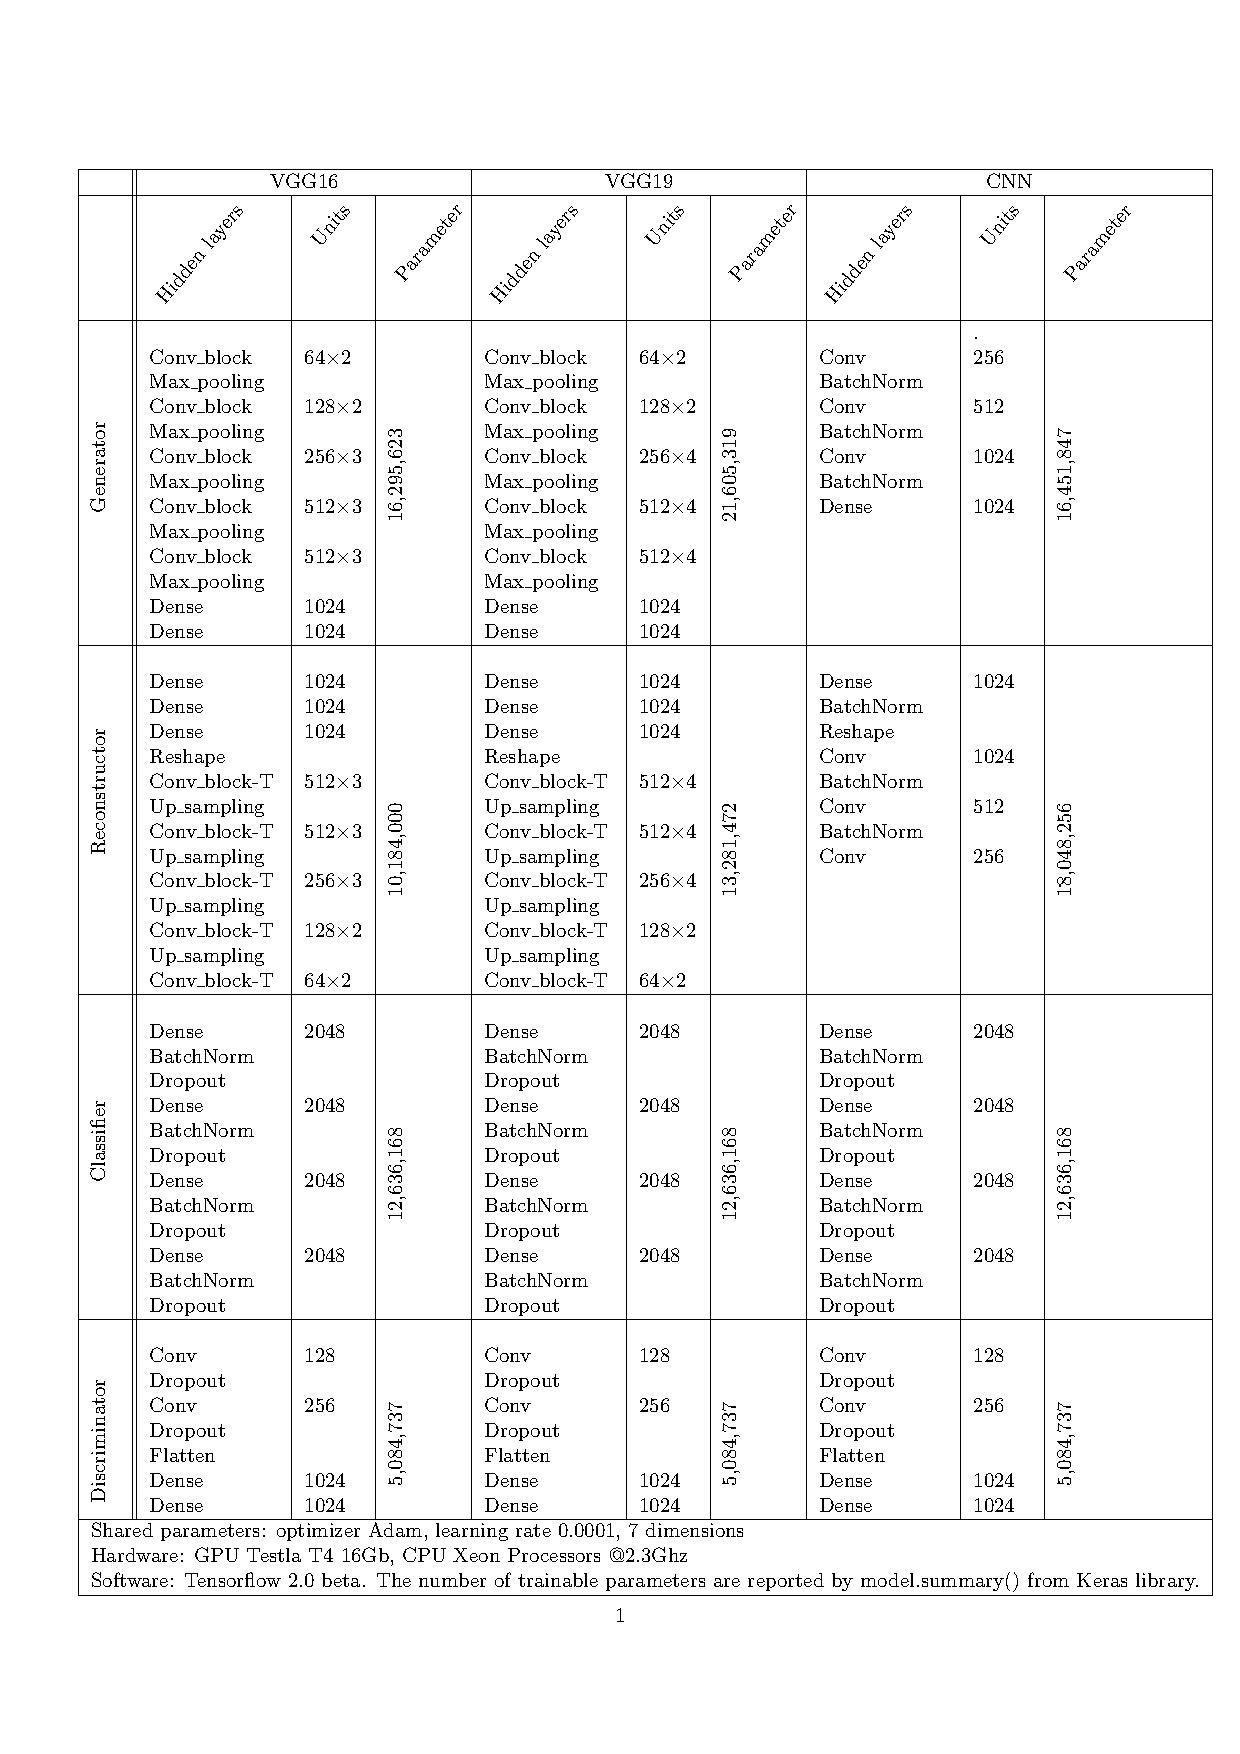
\includegraphics[width=0.7\linewidth, trim=1cm 2.5cm 0.1cm 2.5cm, clip=true]{tables/implement_table}
	\caption{Implementation information}
	\label{table:implementation}
\end{table}

To evaluate the reliability, we test our framework with different levels of authentication corresponding to binary classification (single-level) and multi-class classification (multi-level). For the single-level authentication system, we consider half of the subjects in the dataset are valid to access company's resources while the rest are invalid. We randomly divide the dataset into two groups of subjects and labels their images to (1) or (0) depending on their access permission. For the cases of multi-level authentication system, we divide the subjects into four groups and eight groups. Therefore, the authentication server becomes four-class and eight-class classifier respectively. 
\subsection{Utility}
We use accuracy metric to evaluate the utility of dimension-reduced data. The testing dataset is tested with the classifier extracted from our framework. Different structures of Generator and re-constructor are applied including VGG19, VGG16, basic CNN on different privilege levels which correspond to multi-class classification. Figure \ref{fig:acc} illustrates the accuracies for different dimensions from three to seven over the three facial datasets. Overall, the accuracies improve when the number of dimension increases. The accuracies on the two gray image datasets (AT\&T and Yale\_B) reaches 90\% and higher when using VGG with only seven dimensions. This accuracy figure for Celeba is smaller, but it still reaches 80\%. In general, VGG19 structure performs better than using VGG16 and basic CNN in terms of utility due to the complexity (table \ref{table:implementation}) and adaptability to image datasets of VGG19. As the dimension number is reduced from 4,096 (64$\times$64) to 7, we can achieve a compression ratio of 585 yet achieve accuracy of 90\% for the two gray datasets and 80\% for the color dataset. This implies our method could gain a high compression ratio and maintain a high utility in terms of accuracy. During conducting experiments we also observe that the accuracy could be higher if we keep the original resolution of images. However, for convenience and reducing the complexity of our structure, we resize images to the size of 64$\times$64 pixels.    

\subsection{Privacy}
In this study, the Euclidean distance is used to measure the distance between original and reconstructed images: $dist(x,\hat{x}) = ||x-\hat{x}||^2$. Figure \ref{fig:distresult} illustrates the average distances between original images and reconstructed images on testing data with different $\epsilon$ constraints (other setting parameters: seven dimensions, single-level authentication, and VGG19 structure). The achieved distances (red lines) are larger than the hyper-parameter $\epsilon$ (black dotted lines) where $\epsilon$ is less than 0.035 for AT\&T, 0.052 for YaleB and 0.067 for CelebA. Thus, our framework can satisfy $\epsilon$-DR with $\epsilon$ of above values. Due to the fact that the re-constructor obtained some information (we consider the adversary can reach the model and the training data), we can only set the distance constraint $\epsilon$ within a certain range as shown in \ref{fig:distresult}. The intersection between the red line and the dotted black line points out the largest distance our framework can achieve. Since the mean of the target distribution is set to be the same as the mean of training dataset, reconstructed images will be close to the mean of training dataset which we believe it will enlarge the distance and expose less individual information. Thus, the range of epsilon can be estimated base on the expectation of the distance between testing samples and the mean of training data. In addition, the first section of Table \ref{table:visualization} demonstrates some samples and their corresponding reconstructions in single-level authentication and seven dimensions with different achieved accuracies and distances. The reconstructed images could be nearly identical, thus making it visually difficult to recognize the identity of an individual.      
 
\setcounter{figure}{3}	
\begin{figure*}[ht!]
	\begin{subfigure}{.33\textwidth}
		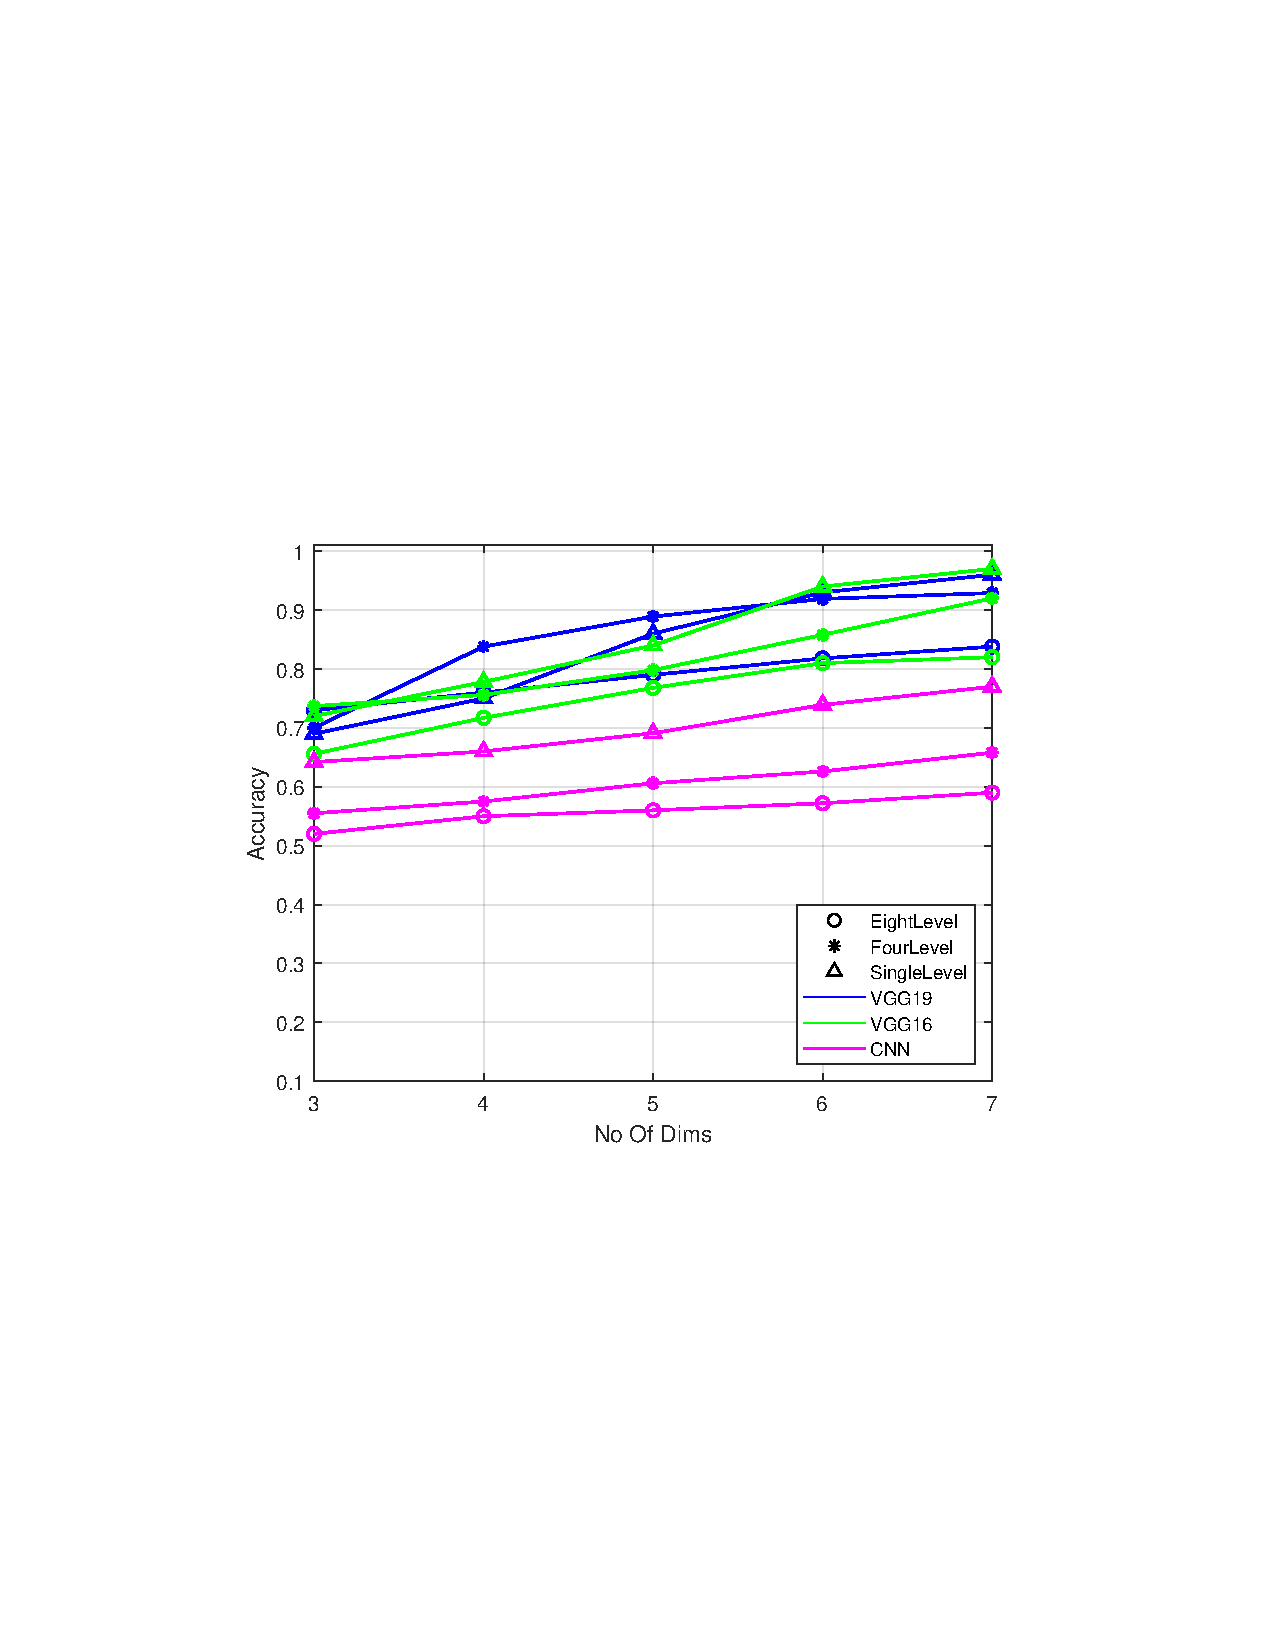
\includegraphics[width=\linewidth, trim=3.8cm 8cm 4cm 8cm, clip=true]{figures/att_acc}
		\captionsetup{justification=centering}
		\caption{ AT\&T}
		\label{fig:att_acc}
	\end{subfigure}
	\begin{subfigure}{.33\textwidth}
		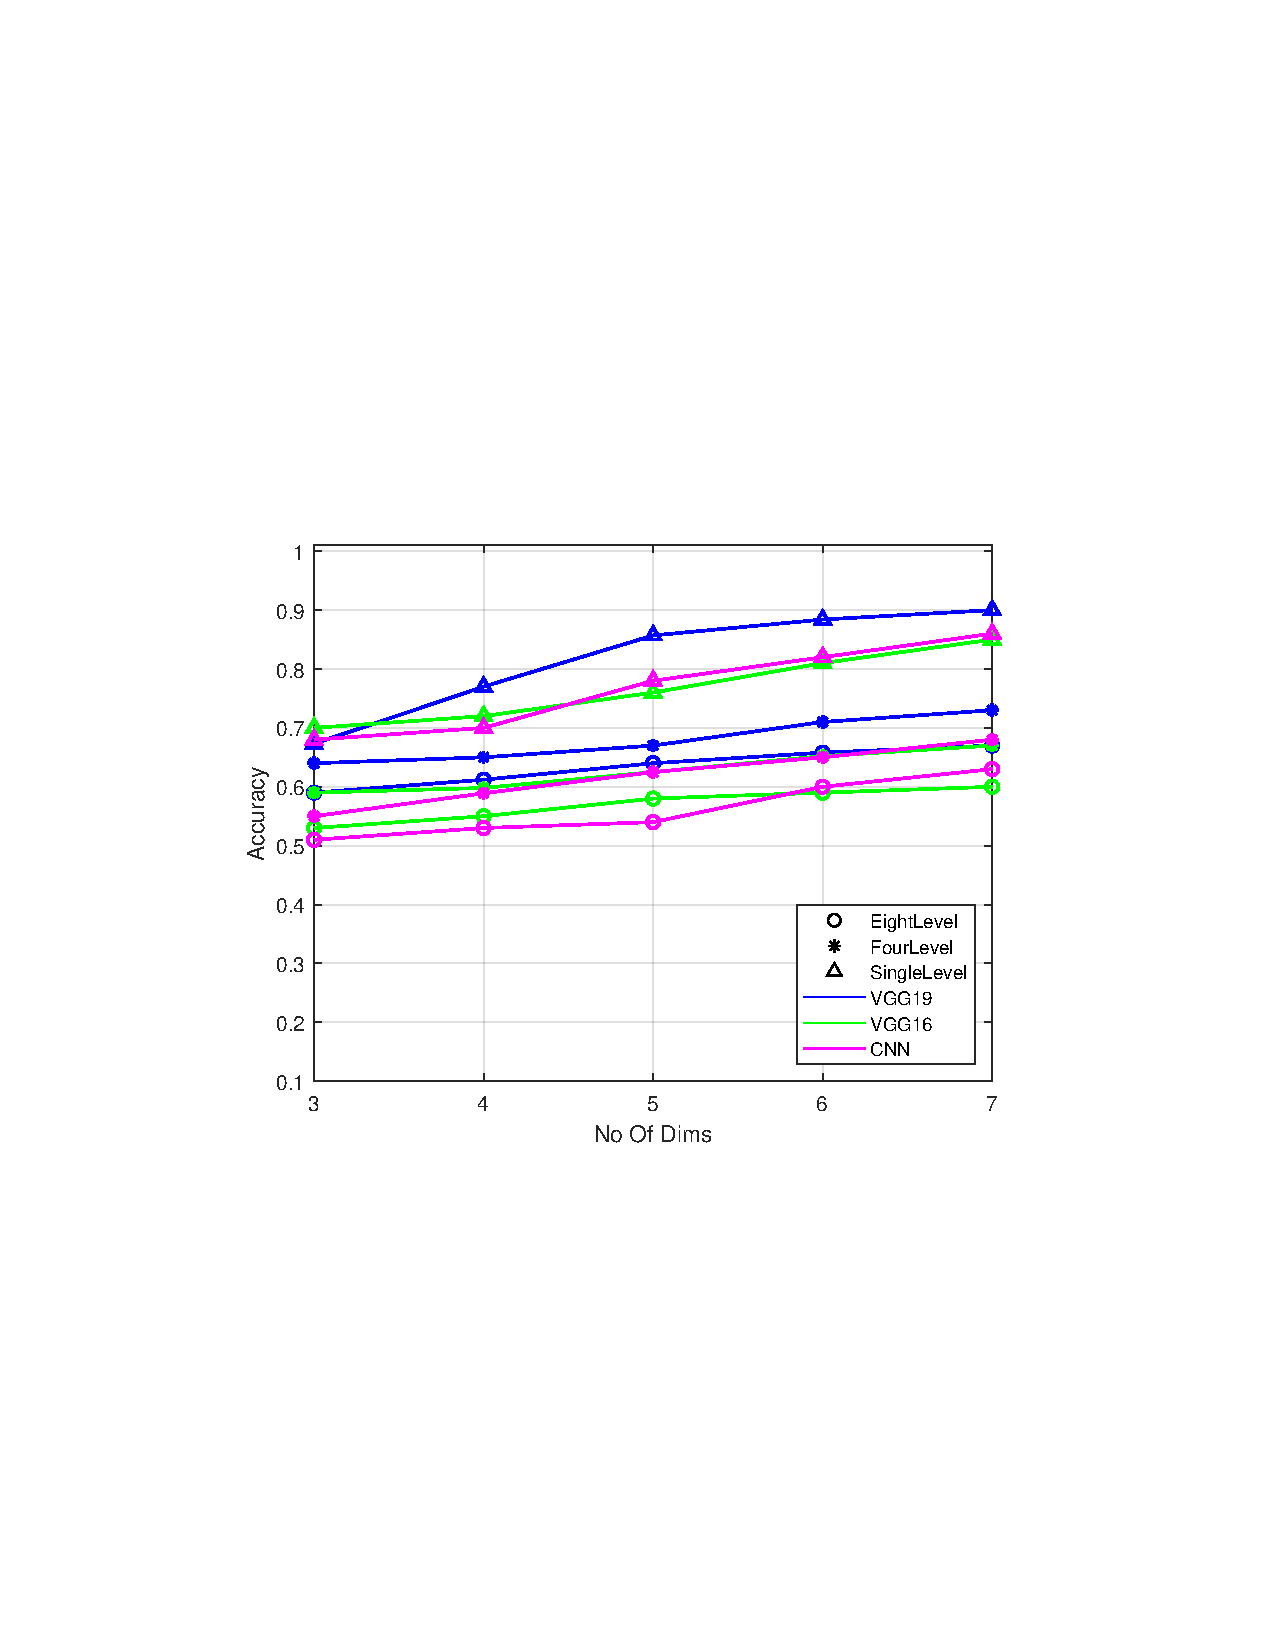
\includegraphics[width=\linewidth, trim=3.8cm 8cm 4cm 8cm, clip=true]{figures/yale_acc}
		\captionsetup{justification=centering}
		\caption{Yale\_B}
		\label{fig:yale_acc}
	\end{subfigure}
	\begin{subfigure}{.33\textwidth}
		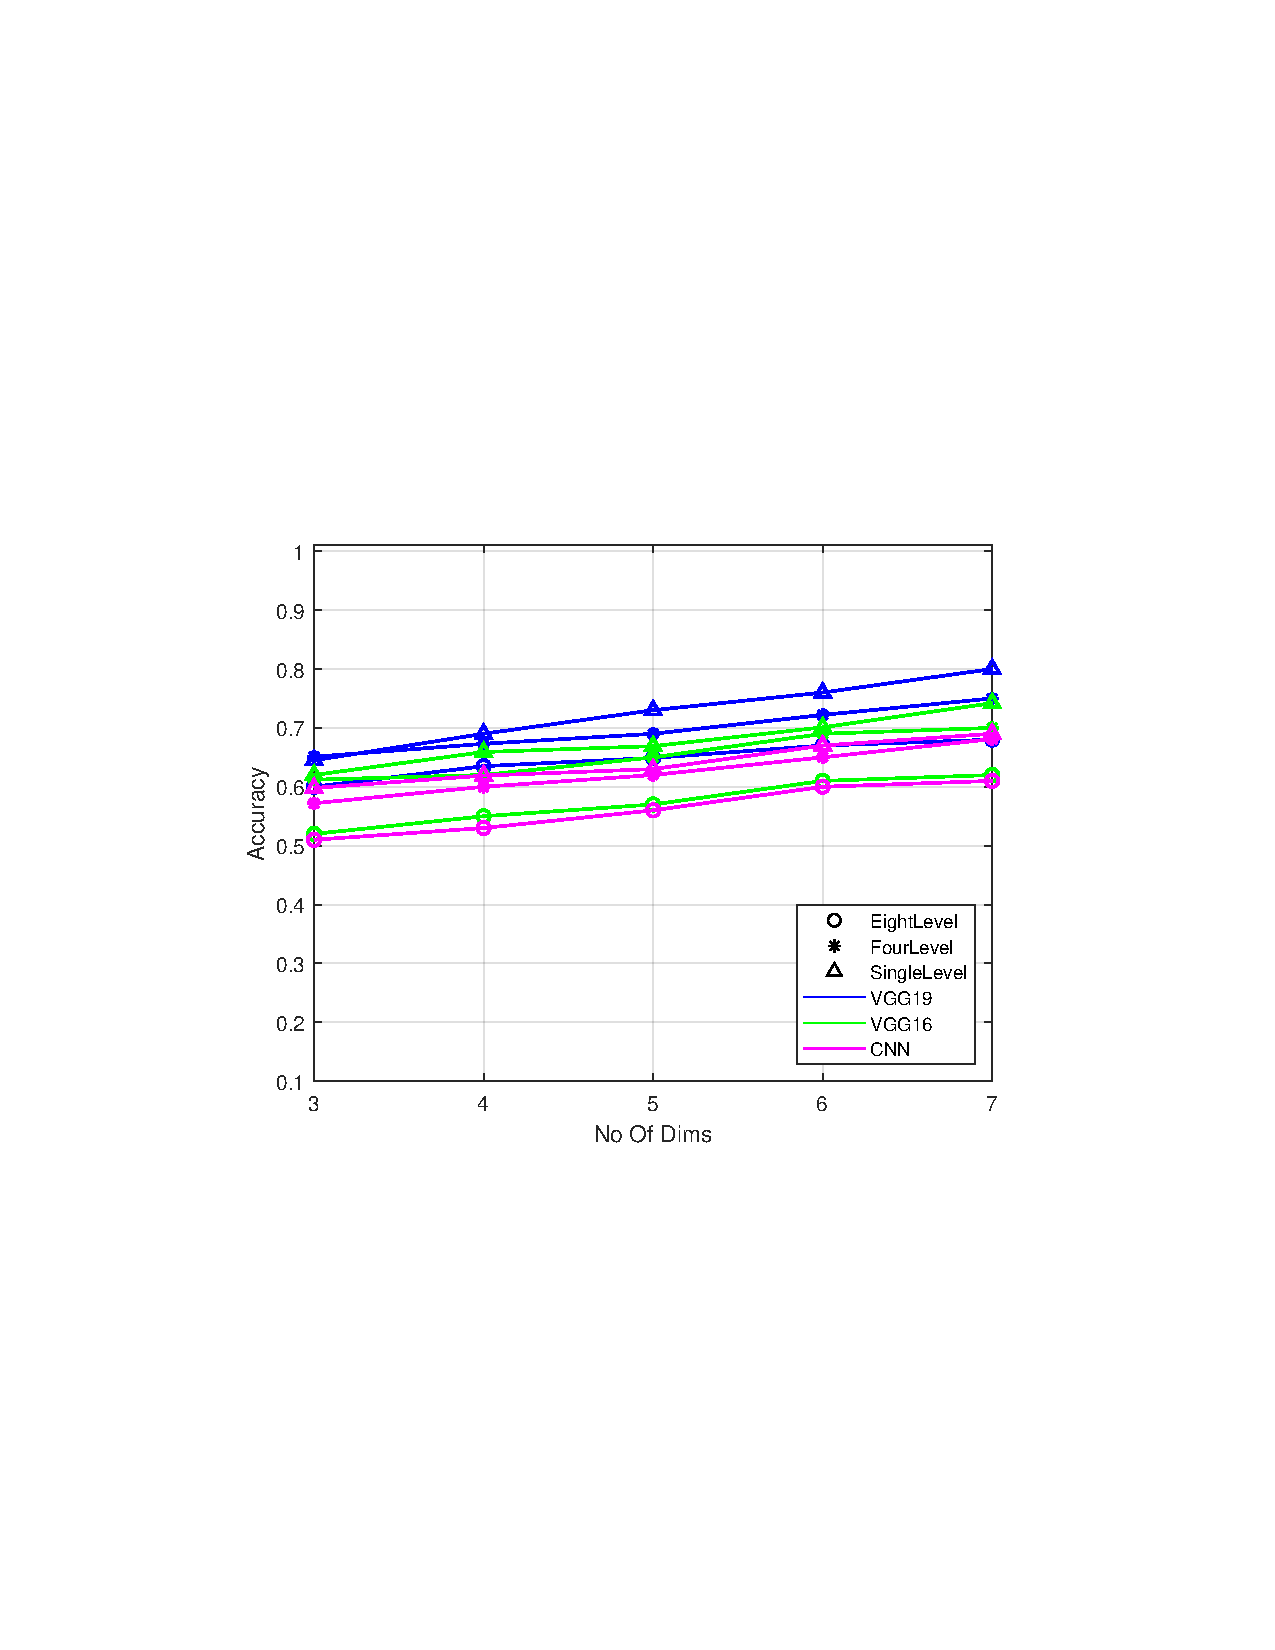
\includegraphics[width=\linewidth, trim=3.8cm 8cm 4cm 8cm, clip=true]{figures/celeba_acc}
		\captionsetup{justification=centering}
		\caption{CelebA}
		\label{fig:celeba_acc}
	\end{subfigure}
	\caption{Accuracy for Different Number of Reduced Dimensions }
	\label{fig:acc}
\end{figure*}

\begin{figure*}[ht!]
	\begin{subfigure}{.33\textwidth}
		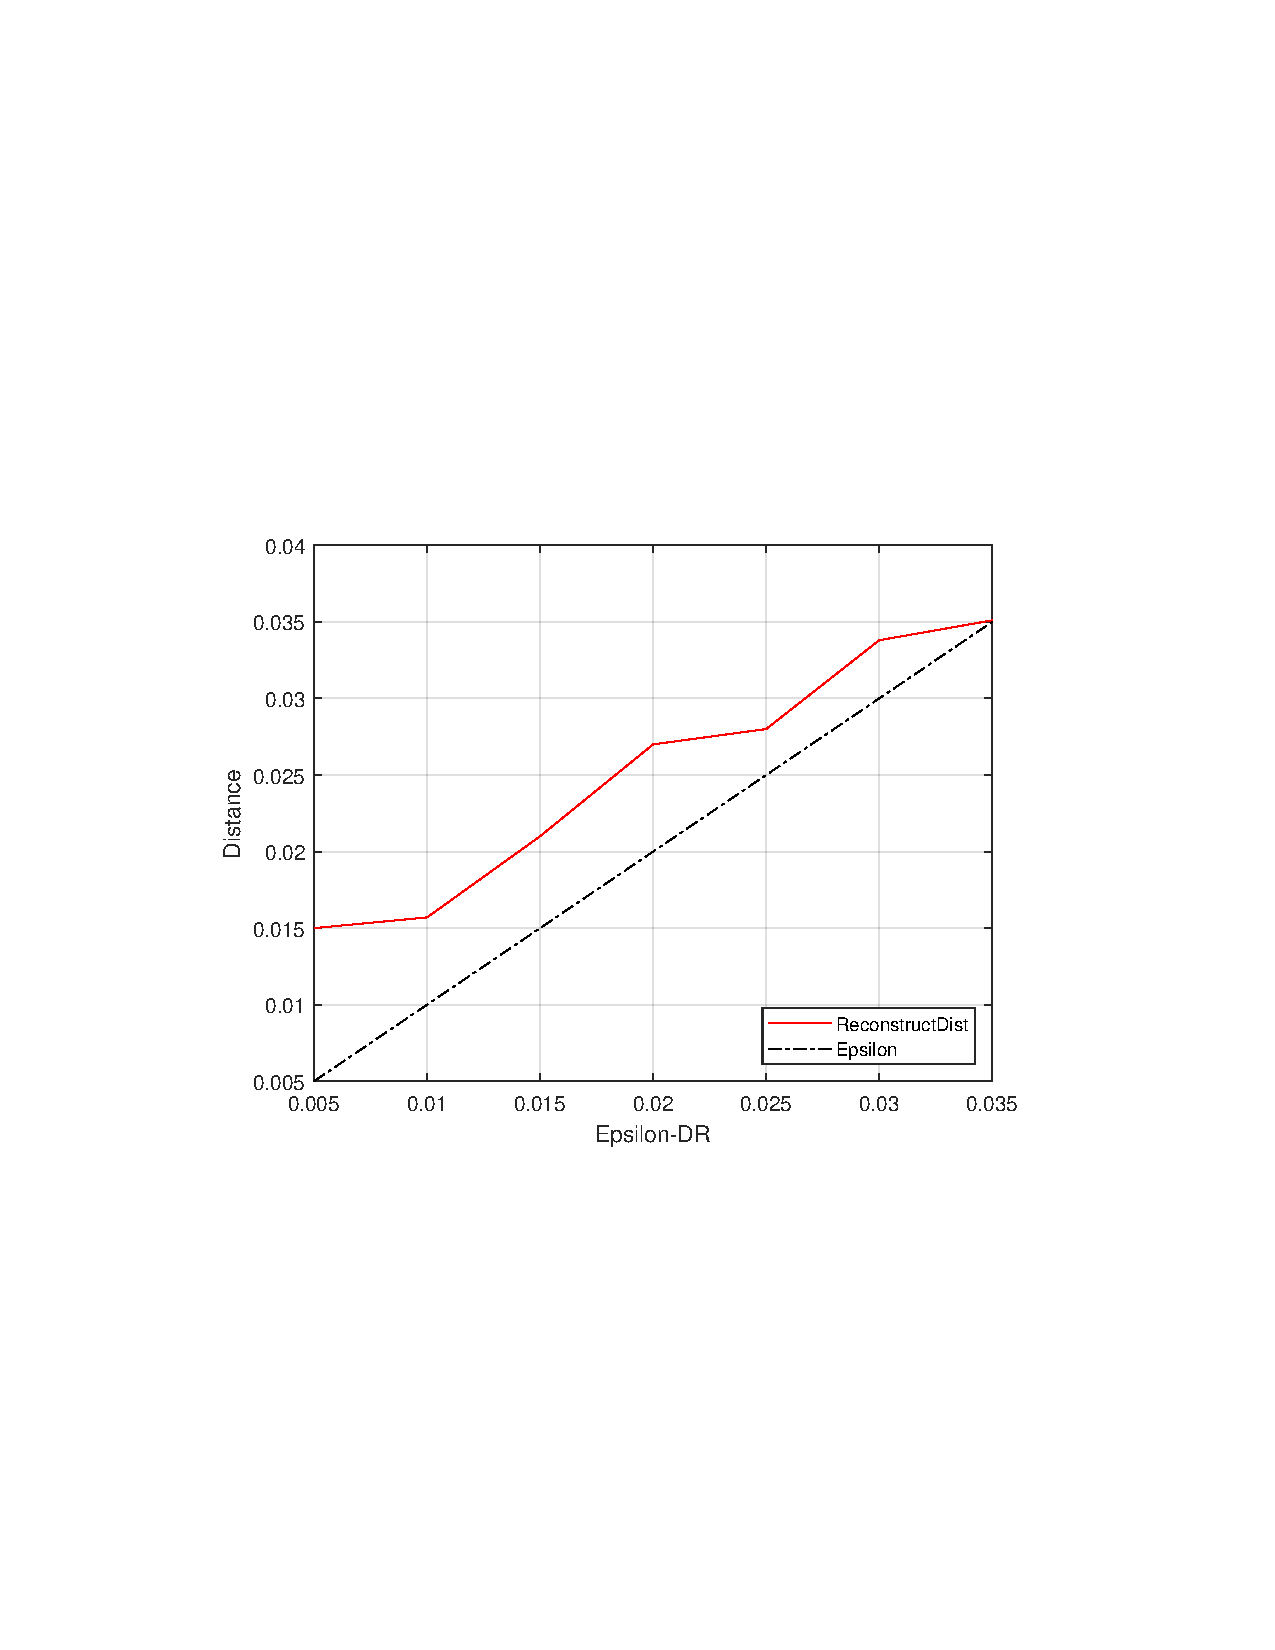
\includegraphics[width=\linewidth, trim=3.8cm 8cm 4cm 8cm, clip=true]{figures/ep_att}
		\captionsetup{justification=centering}
		\caption{ AT\&T}
		\label{fig:att_dist}
	\end{subfigure}
	\begin{subfigure}{.33\textwidth}
		\includegraphics[width=\linewidth, trim=3.8cm 8cm 4cm 8cm, clip=true]{figures/ep_yale}
		\captionsetup{justification=centering}
		\caption{Yale\_B}
		\label{fig:yale_dist}
	\end{subfigure}
	\begin{subfigure}{.33\textwidth}
		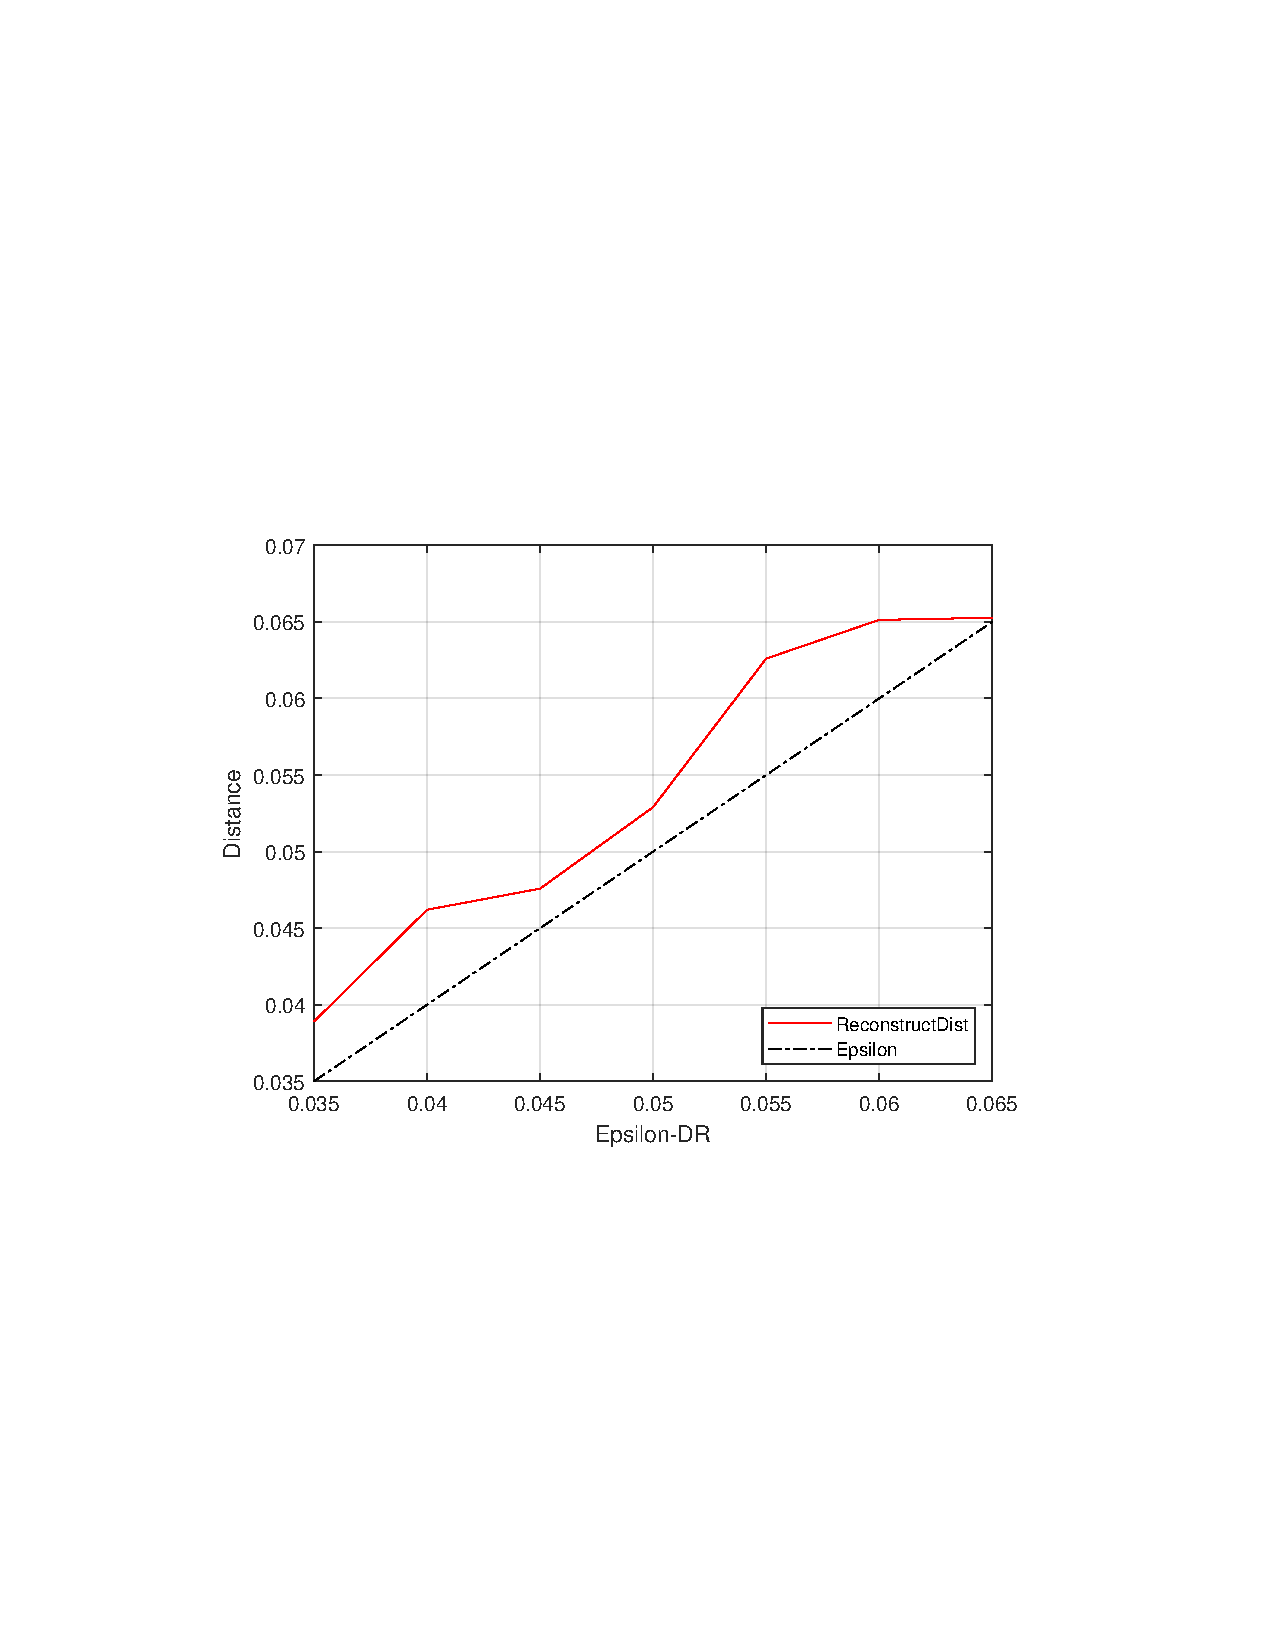
\includegraphics[width=\linewidth, trim=3.8cm 8cm 4cm 8cm, clip=true]{figures/ep_celeba}
		\captionsetup{justification=centering}
		\caption{CelebA}
		\label{fig:celeba_dist}
	\end{subfigure}
	\caption{Average Distance Measurement Result \{ 7 dimensions, Single-Level\}}
	\label{fig:distresult}
\end{figure*}
"


\setcounter{section}{5} "
\section{Visual Comparison to Privacy Preserving Techniques }
\label{AutoGAN_DP_PCA}

In this section, we compare AutoGAN-DRP with other privacy preserving methods in terms of ability to visually identify client's identities. We choose the widely used tool for privacy preserving Differential Privacy (DP) [27] and another privacy preservation method utilizing dimensionality reduction technique (i.e., Principle Component Analysis [34] ).

In these experiments, we implement AutoGAN-DRP following VGG19 structure for the Generator and Re-constructor, and other setting parameters (e.g., number of hidden layers, learning rate, optimization) are shown in Table \ref{table:implementation}. The images are reduced to seven dimensions for different values of $\epsilon$-DR to achieve different distances and accuracies. The datasets are grouped into two groups corresponding to a binary classifier. 

For implementing DP, we first generate a classifier on the authentication server by training the datasets with a VGG19 binary classifier (the structure of hidden layers is similar to our Generator in Table \ref{table:implementation}). The testing images are then perturbed using differential privacy method. Specifically, Laplace noise is added to the images with the sensitivity coefficient of 1 (it is computed by the maximum range value of each pixel [0,1]) and different DP epsilon parameters (this DP epsilon is different from our $\epsilon$-DR). The perturbed images are then sent to the authentication server and fed to the classifier. We visually compare the perturbed images of this method with AutoGAN. 

In addition, we follow instruction in FRiPAL [11] in which the clients reduce image dimension using Principle Component Analysis (PCA) and send reduced features to the server. FRiPAL claims that by reducing image dimension, their method can be more resilient to reconstruction attacks. The experiments are conducted with different number of reduced dimension. The images are reconstructed using \textit{Moore–Penrose inverse} method with assumption that an adversary has assess to the model. The classification accuracy is evaluated using a classifier which has similar structure to AutoGAN's classifier. 

Table \ref{table:visualization} shows image samples and results over the three datasets. Overall, AutoGAN-DRP is more resilient to reconstruction attacks compared to the other two techniques. For instance, at the accuracy of 79\% on AT\&T dataset, 80\% on YaleB, and 73\% on CelebA, we cannot distinguish entities from the others. For DP method, the accuracy decreases when the DP epsilon decreases (adding more noise), and the perturbed images become harder to recognize. However, at a low accuracy 57\%, we are still able to distinguish identities by human eyes. The reason is that DP noise does not focus on the important visual pixels. For PCA, the accuracy also goes down when the number of dimensions decreases and the distances increase. Since PCA transformation is linear and deterministic, the original information can be significantly reconstructed using the inverse transformation deriving from the model or training data. Thus, at the accuracy of 75\% on AT\&T, 71\% on YaleB, and 68\% on CelebA, we still can differentiate individuals. Overall, our proposed method shows the advantage in securing the data while retaining high data utility.       
\\ 
\setcounter{table}{1}

\begin{table}[H]
	\centering
	%trim  left, bottom, right and top 
	\includegraphics[width=0.8\linewidth, trim=1cm 3cm 1cm 3cm, clip=true]{tables/img_table}
	\caption{Sample visualization of AutoGAN, DP, PCA over three datasets}
	\label{table:visualization}
\end{table}

" \\ \\


\color{blue}
\underline{Comment 1.2}
My concern is enhanced by the fact that I could not find the precise information on the neural network architectures used in the study.

\color{black}
\underline{Response:}

In the revision, we added table \ref{table:implementation} and provided more information on neural network architectures in section 4.1 (Experiment setup) as follows.\\ 
	"
	The generator and re-constructor in Figure \ref{fig:eGAN} are implemented by three different structures. Specifically, we follow the architecture of recent powerful models VGG19, VGG16 [33] and a basic convolutional network (CNN). We modify the models to adapt to our data size (64$\times$64). Discriminator and Classifier are built on fully connected neural network and convolutional network respectively. Leaky ReLU is used for activation function in hidden layers. We use linear activation function for generator's output layers and softmax activation functions for other components' output layers. Each component is trained in 5 local iterations ($n_r, n_g, n_d, n_c$), and the entire system is trained in 500 global iterations ($n$). The target distribution is drawn from Gaussian distribution (with the covariance value of 0.5 and the mean is the average of the training data). Table \ref{table:implementation} provides detail information of neural networks' structures and other implementation information.  "
	
	\setcounter{table}{0}
	\begin{table}[H]
		\centering
		%trim  left, bottom, right and top 
		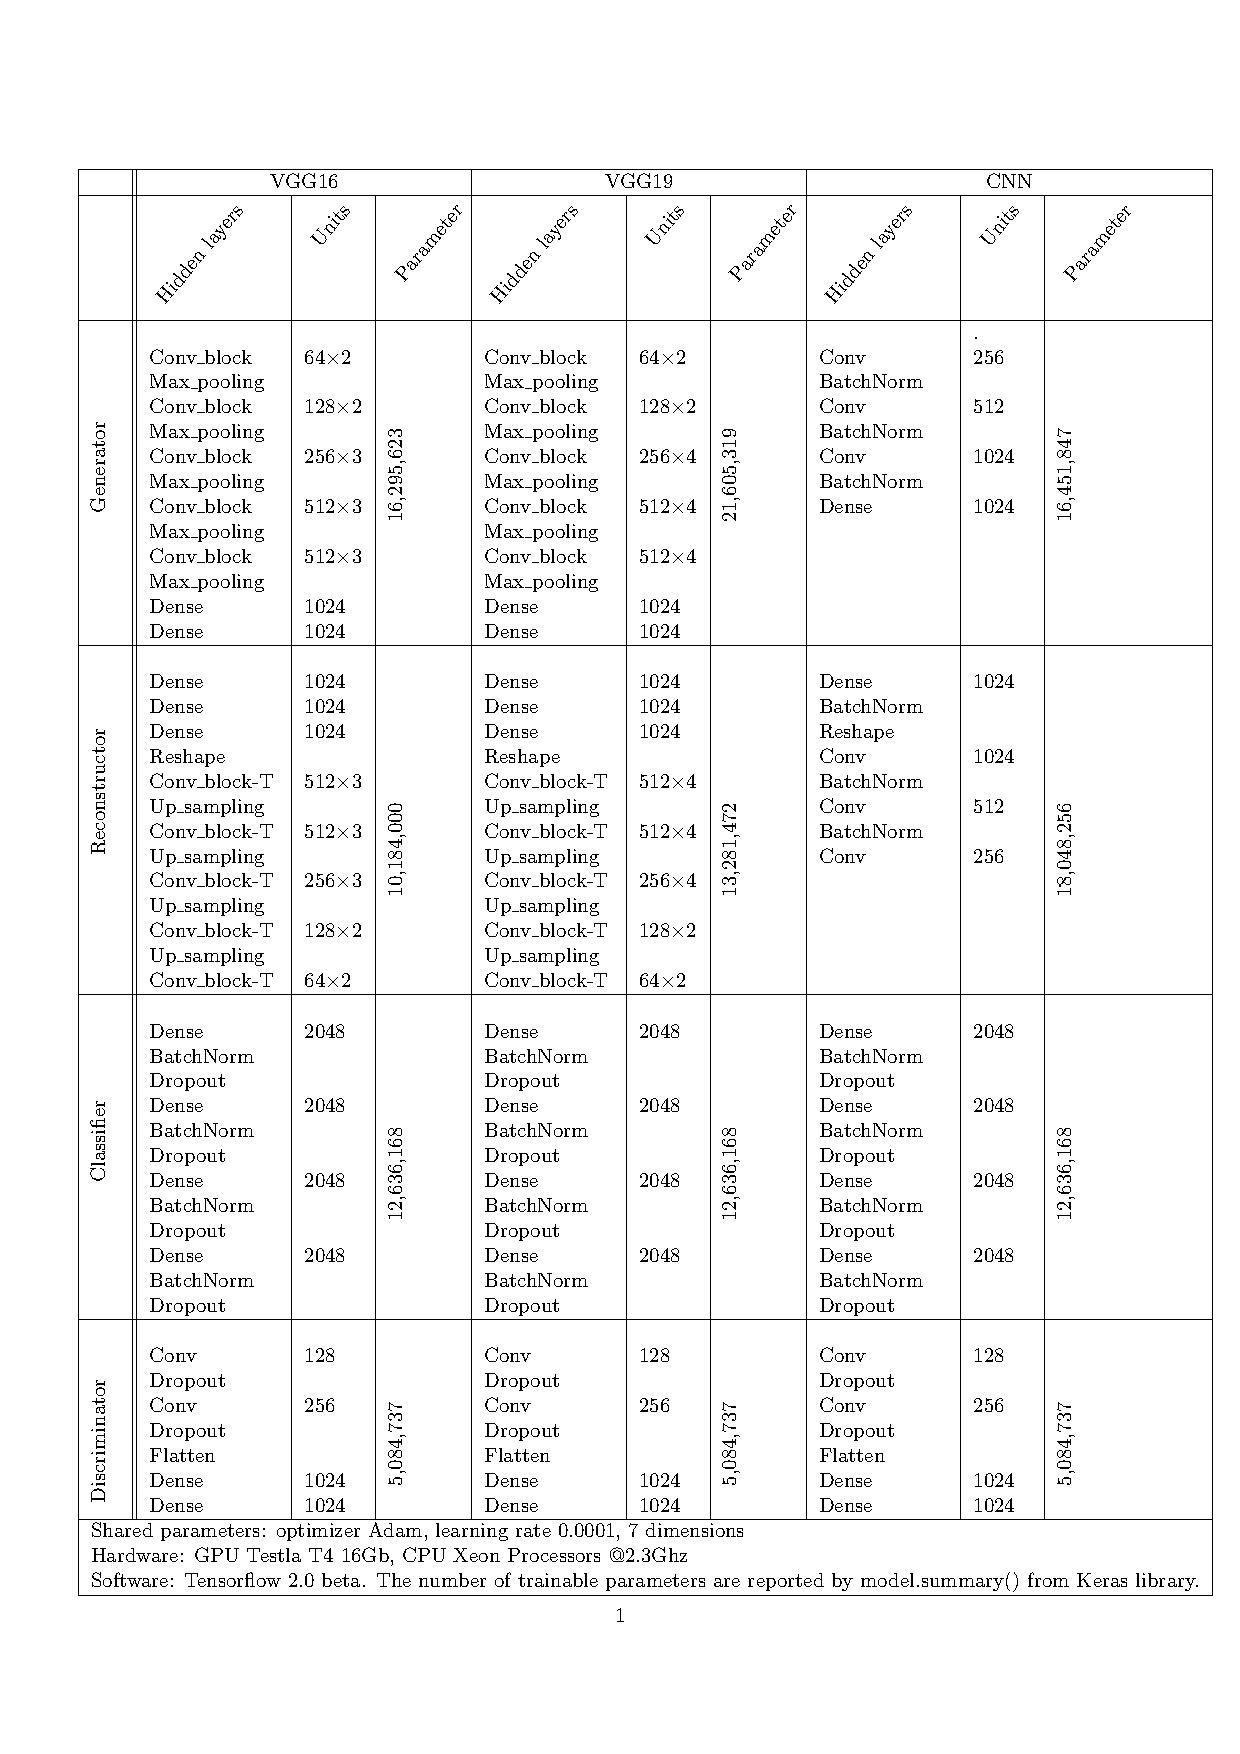
\includegraphics[width=0.7\linewidth, trim=1cm 2.5cm 0.1cm 2.5cm, clip=true]{tables/implement_table}
		\caption{Implementation information}
		\label{table:implementation}
	\end{table}
	
	
	
	%%%%%%%%%%%%%%%%%%%%%%%%%%%%%%%%%%%%%%%%%%%%%%%%%%%%%%%%%%%%%%%%%%%%%%%%%%%%%%%%%
\newpage
\begin{enumerate}[II.]
	\item RESPONSE TO REVIEWER 2
\end{enumerate}
The authors would like to express sincere thanks to the reviewer for the thorough and constructive
comments. In what follows, we present detailed comments in response to the individual points raised by
the reviewer and elaborate on how the manuscript has been revised.

\color{blue}
\underline{Comment 2.1}
This paper proposed a dimension reduction-based method for privacy preservation. However, there are some problems.\\
1. The organizational structure of the article is unreasonable, section 2, section 3 and section 4 should be introduced in the introduction and related work. I hope it can improve readability.

\color{black}
\underline{Response:}

Thank you for the insightful comment. \\
1. As recommended, in this revision we merged Section 3 (Preliminary) into Section 2 (Related Work).\\ 
2. The problem was introduced in the introduction. However, to clarify the problem and provide a comprehensive scenario for the problem, we formally introduced again the problem in Section 4. For this reason, in the revision  Section 4 (Problem) and Section 5 ($\epsilon$-Dimension Reduction Privacy) were merged to the top of Section 6 (Methodology). Thus, we hope the changes can support the readability of our methodology. \\


\color{blue}
\underline{Comment 2.2}
Please briefly describe the content in Figure 1, which will be more helpful for readers to understand.


\color{black}
\underline{Response:}
\setcounter{figure}{0}
\begin{figure}[H]
	\centering
	\includegraphics[width=0.5\linewidth]{supplement/AttackModel_CP}
	\captionsetup{justification=centering}
	\caption{Attack Model}
	\label{fig:attackmodel}
\end{figure} 	
Thank you for your insightful comment. In the revision, we clarify Figure \ref{fig:attackmodel} in the problem statement section (Section 3.1.1) as follows. 

	"
	\dots We introduce the problem through the practical scenario mentioned in Section \ref{sec:introduction}. Figure \ref{fig:attackmodel} briefly describes the entire system in which staff members (clients) in a company request access to company resources, such as websites and data servers through a face recognition access control system. For example, if member n requests to access web server 2, the local device first takes a facial photo of the member by an attached camera, locally transforms it into lower dimension data, and sends to an authentication center. The authentication server then obtains the low dimensional data and determines member access eligibility by using a classifier without clear face images of the requesting member. We consider that the system has three levels of privileges (i.e., single level, four-level, eight-level) corresponding to three groups of members. We assume the authentication server is semi-honest (it obeys work procedure but might be used to infer personal information). If the server is compromised, an adversary in the authentication center can reconstruct the face features to achieve plain-text face images and determine members' identity.  
"\\\\
  


\color{blue}
\underline{Comment 2.3}
Please explain what is the operation of E[] in equation (1)?

\color{black}
\underline{Response:}

In the revision, Equation (1) was indexed as Equation (3), and we added explanation for this equation as follows.\\
"
\setcounter{equation}{2}
\begin{equation}
\label{eq:modularity}
\mathbb{E}[dist(x, \hat{x})] \geq \epsilon
\end{equation}
where $\mathbb{E}[\cdot]$ is the expectation, $\epsilon \geq 0$, $x^{\prime}=F(x)$, $\hat{x}=R(x^{\prime})$, and $R(\cdot)$ is the Reconstruction Function.
" \\

\color{blue}
\underline{Comment 2.4}
Please explain which method is used to project original data to low dimensional space?

\color{black}
\underline{Response:}

Our method leverages dimension reduction technique using an Auto-encoder and feedback from other components (the classifier and discriminator) in our framework to project data onto a latent space.  

In this revision, we clarify and provide more detail on the method used to project data to lower dimension space in Section 3.4 (AutoGAN-based Dimension Reduction for Privacy Preserving) as follows.


	"
	We propose a deep learning framework for transforming face images to low dimensional data which is hard to be fully reconstructed. The framework can be presented in Figure \ref{fig:eGAN}. We leverage the structure of an auto-encoder [22] which contains encoder and decoder (in this work, we called them generator and re-constructor) in order to reduce data dimension. More specifically, the low dimensional representations are extracted from the middle layer of the auto-encoder (the output of the generator). The dimension-reduced data can be sent to the authentication server as an authentication request. We consider an adversary as a re-constructor implemented by a decoder. To resist against fully reconstructing images, the framework utilizes a discriminator in GAN [21] to direct reconstructed data to a designated target distribution with an assumption that the target distribution is different from our data distribution. In this work, the target distribution is sampled from Gaussian distribution and the mean is the average of training data. After projecting data into a lower dimension domain, the re-constructor is only able to partially reconstruct the data. Therefore, the adversary might not be able to recognize an individual's identity. To maintain data utility, we also use feedback from a classifier. The entire framework is designed to enlarge the distance between original data and its reconstruction to preserve individual privacy and retain significant data information. The dimension-reduced transformation model is extracted from the framework and provided to clients for reducing their face image dimensions. The classification model will be used in an authentication center that classifies whether a member's request is valid to have access (1) or not (0). 
	"

\color{blue}
\underline{Comment 2.5}
Please explain how to estimate the range of values of epsilon ?


\color{black}
\underline{Response:}

In this study, the distance is defined as the L2 norm distance between the original data and reconstructed data. In this revision we added our observation in order to estimate the range of $\epsilon$ to Section 4 (Experiment and Discussion) as follows.  

" 
\dots Since the mean of the target distribution is set to be the same as the mean of training dataset, reconstructed images will be close to the mean of training dataset which we believe it will enlarge the distance and expose less individual information. Thus, the range of epsilon can be estimated base on the expectation of the distance between testing samples and the mean of training data.\dots
"\\


\color{blue}
\underline{Comment 2.6}
There are few methods for comparing experiments, no convincing. More recent methods should be used in the comparison experiments. In addition, computation complexity or time consumption of the methods should also be given. I hope this will help to improve the quality of the paper.

\color{black}
\underline{Response:}


In this revision we conducted more experiments using most current powerful structure of convolution networks (i.e., VGG16, VGG19 [32], basic CNN) for the Generator and their inverted structures for the Reconstructor. By examining most recent powerful structure of reconstructor, we aim at evaluating strong adversaries who attempt to reconstruct our original data. Beside the comparison with GAP in Section 5, we also conducted more experiments to compare with other privacy preservation techniques (i.e., Differential Privacy, Principle Component Analysis for privacy preservation) in Section 6. In addition, we added Table[1] in Section 4 which provides detail information of used neural networks, number of parameters in each component and hardware, and software information to improve paper quality. 
Section 4 (Experiment and Discussion) is updated, and Section 6 is added as follows.\\


\titleformat*{\subsection}{\normalsize\itshape}
\titleformat*{\section}{\normalsize\itshape}
\setcounter{section}{3}"
\section{Experiments and Discussion}
In this section, we demonstrate our experiments over three popular supervised face image datasets: \textit{the Extended Yale Face Database B} [18], \textit{AT}\&\textit{T} [19], and \textit{CelebFaces Attributes Dataset (CelebA)} [20]. To evaluate our method performance, we also conduct experiments with different generator and re-constructor structures, different types of classifications (binary and multi-class classification), different numbers of reduced dimensions. The effectiveness of the method is then evaluated in terms of utility and privacy.   
\subsection{Experiment Setup}
\textit{The Extended Yale Face Database B} (YaleB) contains 2,470 grayscale images of 38 human subjects under different illumination conditions and their identity label. In this dataset, the image size is 168$\times$192 pixels. The AT\&T dataset has 400 face images of 40 subjects. For convenience, we resize each image of these two dataset to 64$\times$64 pixels. CelebA is a color facial image dataset containing 202,599 images of 10,177 subjects. 1,709 images of the first 80 subjects are used for our experiment. Each image is resized to 64$\times$64$\times$3 pixels. All pixel values are scaled to the range of [0,1]. We randomly select 10\% of each subject's images for validation and 15\% for testing dataset. 

The generator and re-constructor in Figure \ref{fig:eGAN} are implemented by three different structures. Specifically, we follow the architecture of recent powerful models VGG19, VGG16 [33] and a basic convolutional network (CNN). We modify the models to adapt to our data size (64$\times$64). Discriminator and Classifier are built on fully connected neural network and convolutional network respectively. Leaky ReLU is used for activation function in hidden layers. We use linear activation function for generator's output layers and softmax activation functions for other components' output layers. Each component is trained in 5 local iterations ($n_r, n_g, n_d, n_c$), and the entire system is trained in 500 global iterations ($n$). The target distribution is drawn from Gaussian distribution (with the covariance value of 0.5 and the mean is the average of the training data). Table \ref{table:implementation} provides detail information of neural networks' structures and other implementation information. 

\setcounter{table}{0}
\begin{table}[H]
	\centering
	%trim  left, bottom, right and top 
	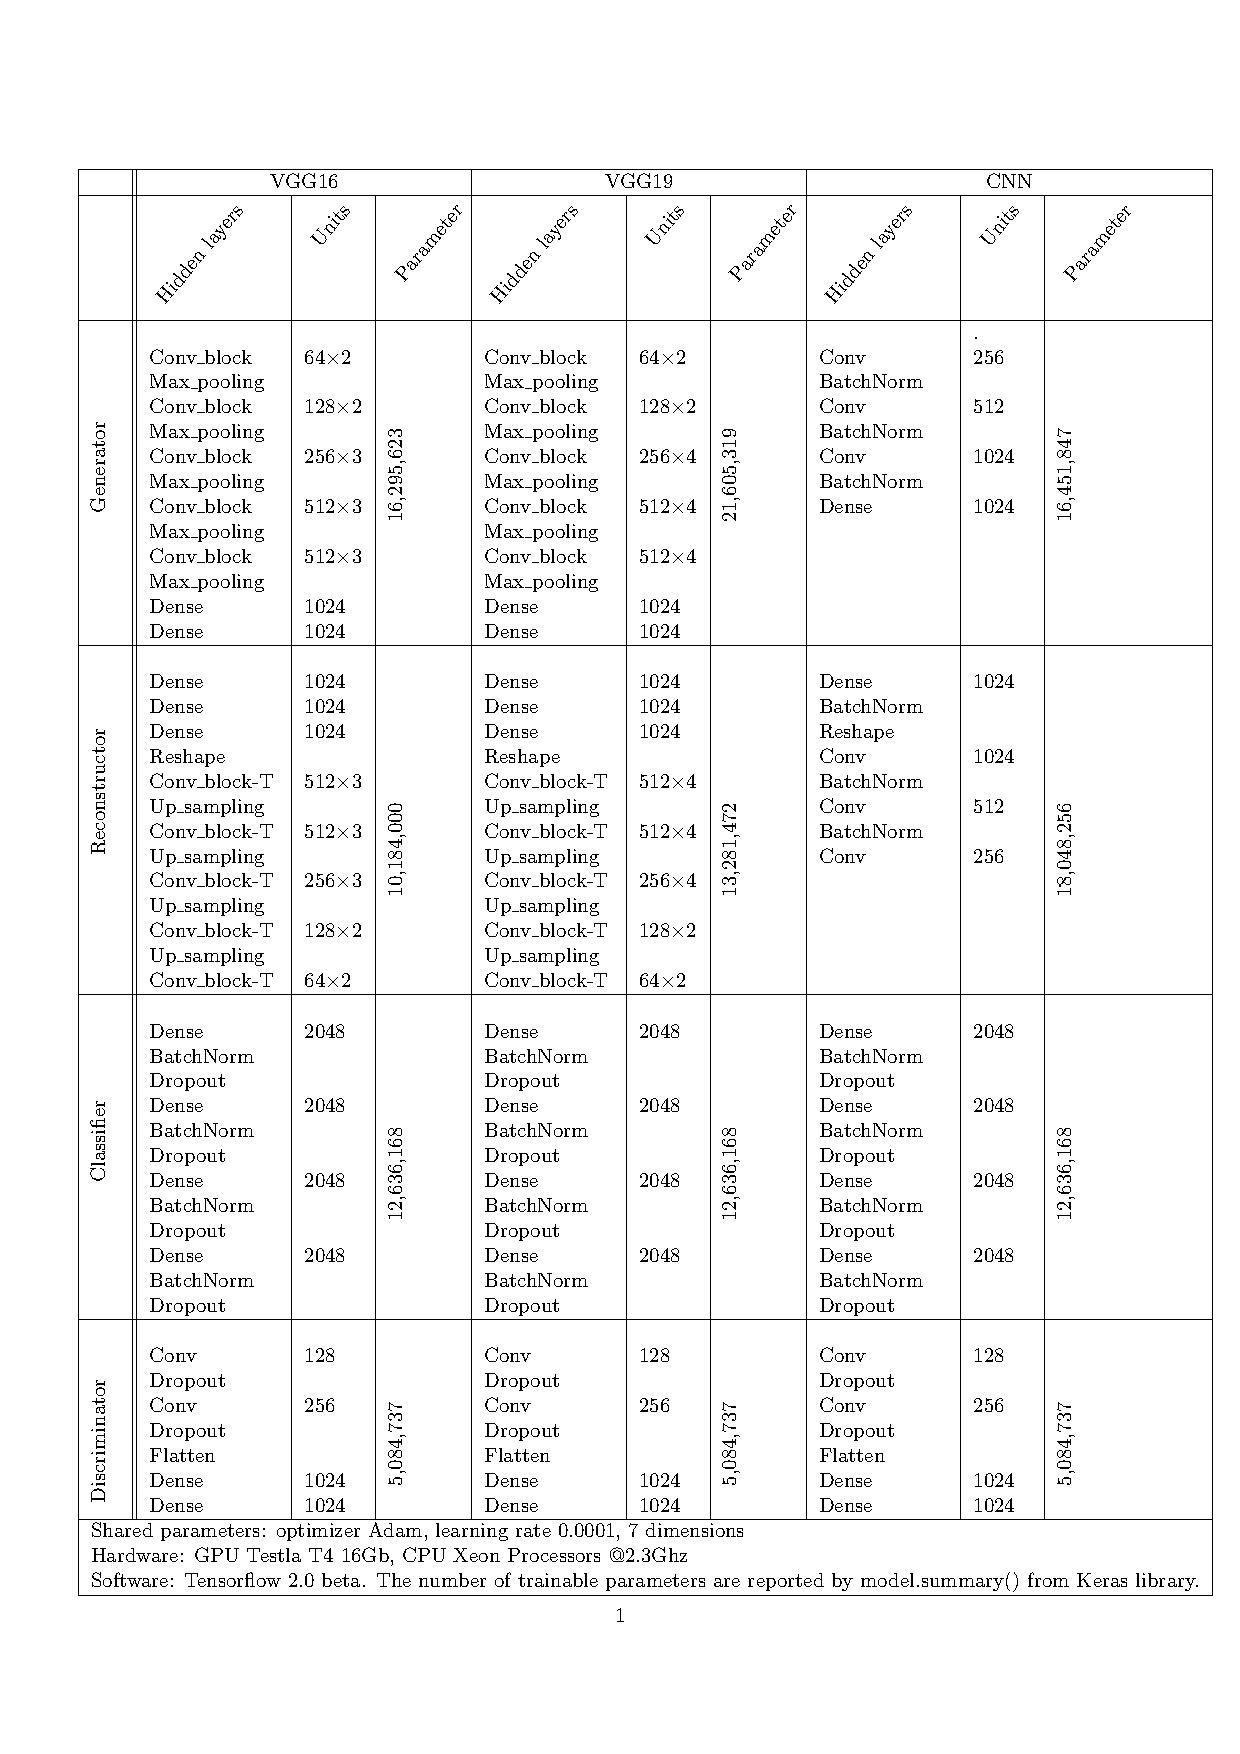
\includegraphics[width=0.7\linewidth, trim=1cm 2.5cm 0.1cm 2.5cm, clip=true]{tables/implement_table}
	\caption{Implementation information}
	\label{table:implementation}
\end{table}

To evaluate the reliability, we test our framework with different levels of authentication corresponding to binary classification (single-level) and multi-class classification (multi-level). For the single-level authentication system, we consider half of the subjects in the dataset are valid to access company's resources while the rest are invalid. We randomly divide the dataset into two groups of subjects and labels their images to (1) or (0) depending on their access permission. For the cases of multi-level authentication system, we divide the subjects into four groups and eight groups. Therefore, the authentication server becomes four-class and eight-class classifier respectively. 
\subsection{Utility}
We use accuracy metric to evaluate the utility of dimension-reduced data. The testing dataset is tested with the classifier extracted from our framework. Different structures of Generator and re-constructor are applied including VGG19, VGG16, basic CNN on different privilege levels which correspond to multi-class classification. Figure \ref{fig:acc} illustrates the accuracies for different dimensions from three to seven over the three facial datasets. Overall, the accuracies improve when the number of dimension increases. The accuracies on the two gray image datasets (AT\&T and Yale\_B) reaches 90\% and higher when using VGG with only seven dimensions. This accuracy figure for Celeba is smaller, but it still reaches 80\%. In general, VGG19 structure performs better than using VGG16 and basic CNN in terms of utility due to the complexity (table \ref{table:implementation}) and adaptability to image datasets of VGG19. As the dimension number is reduced from 4,096 (64$\times$64) to 7, we can achieve a compression ratio of 585 yet achieve accuracy of 90\% for the two gray datasets and 80\% for the color dataset. This implies our method could gain a high compression ratio and maintain a high utility in terms of accuracy. During conducting experiments we also observe that the accuracy could be higher if we keep the original resolution of images. However, for convenience and reducing the complexity of our structure, we resize images to the size of 64$\times$64 pixels.    

\subsection{Privacy}
In this study, the Euclidean distance is used to measure the distance between original and reconstructed images: $dist(x,\hat{x}) = ||x-\hat{x}||^2$. Figure \ref{fig:distresult} illustrates the average distances between original images and reconstructed images on testing data with different $\epsilon$ constraints (other setting parameters: seven dimensions, single-level authentication, and VGG19 structure). The achieved distances (red lines) are larger than the hyper-parameter $\epsilon$ (black dotted lines) where $\epsilon$ is less than 0.035 for AT\&T, 0.052 for YaleB and 0.067 for CelebA. Thus, our framework can satisfy $\epsilon$-DR with $\epsilon$ of above values. Due to the fact that the re-constructor obtained some information (we consider the adversary can reach the model and the training data), we can only set the distance constraint $\epsilon$ within a certain range as shown in \ref{fig:distresult}. The intersection between the red line and the dotted black line points out the largest distance our framework can achieve. Since the mean of the target distribution is set to be the same as the mean of training dataset, reconstructed images will be close to the mean of training dataset which we believe it will enlarge the distance and expose less individual information. Thus, the range of epsilon can be estimated base on the expectation of the distance between testing samples and the mean of training data. In addition, the first section of Table \ref{table:visualization} demonstrates some samples and their corresponding reconstructions in single-level authentication and seven dimensions with different achieved accuracies and distances. The reconstructed images could be nearly identical, thus making it visually difficult to recognize the identity of an individual.      
 
\setcounter{figure}{3}	
\begin{figure*}[ht!]
	\begin{subfigure}{.33\textwidth}
		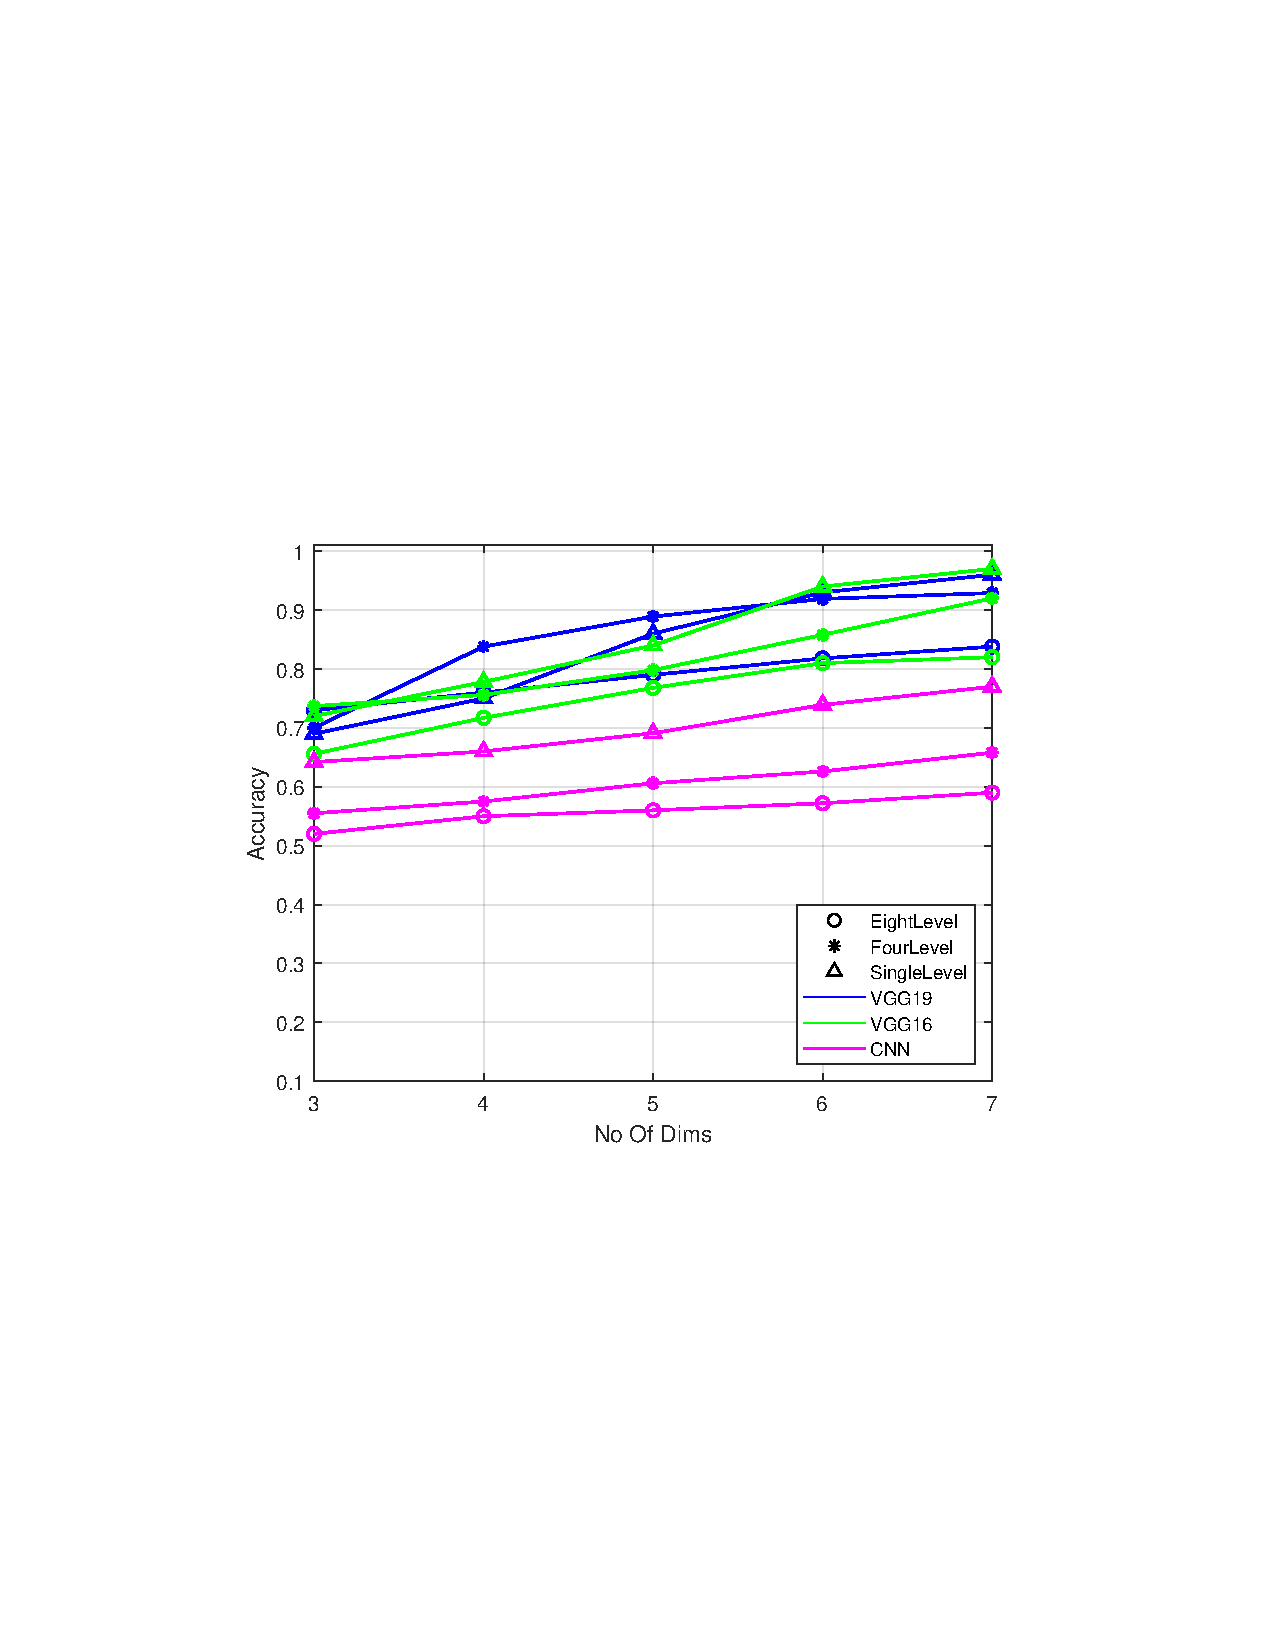
\includegraphics[width=\linewidth, trim=3.8cm 8cm 4cm 8cm, clip=true]{figures/att_acc}
		\captionsetup{justification=centering}
		\caption{ AT\&T}
		\label{fig:att_acc}
	\end{subfigure}
	\begin{subfigure}{.33\textwidth}
		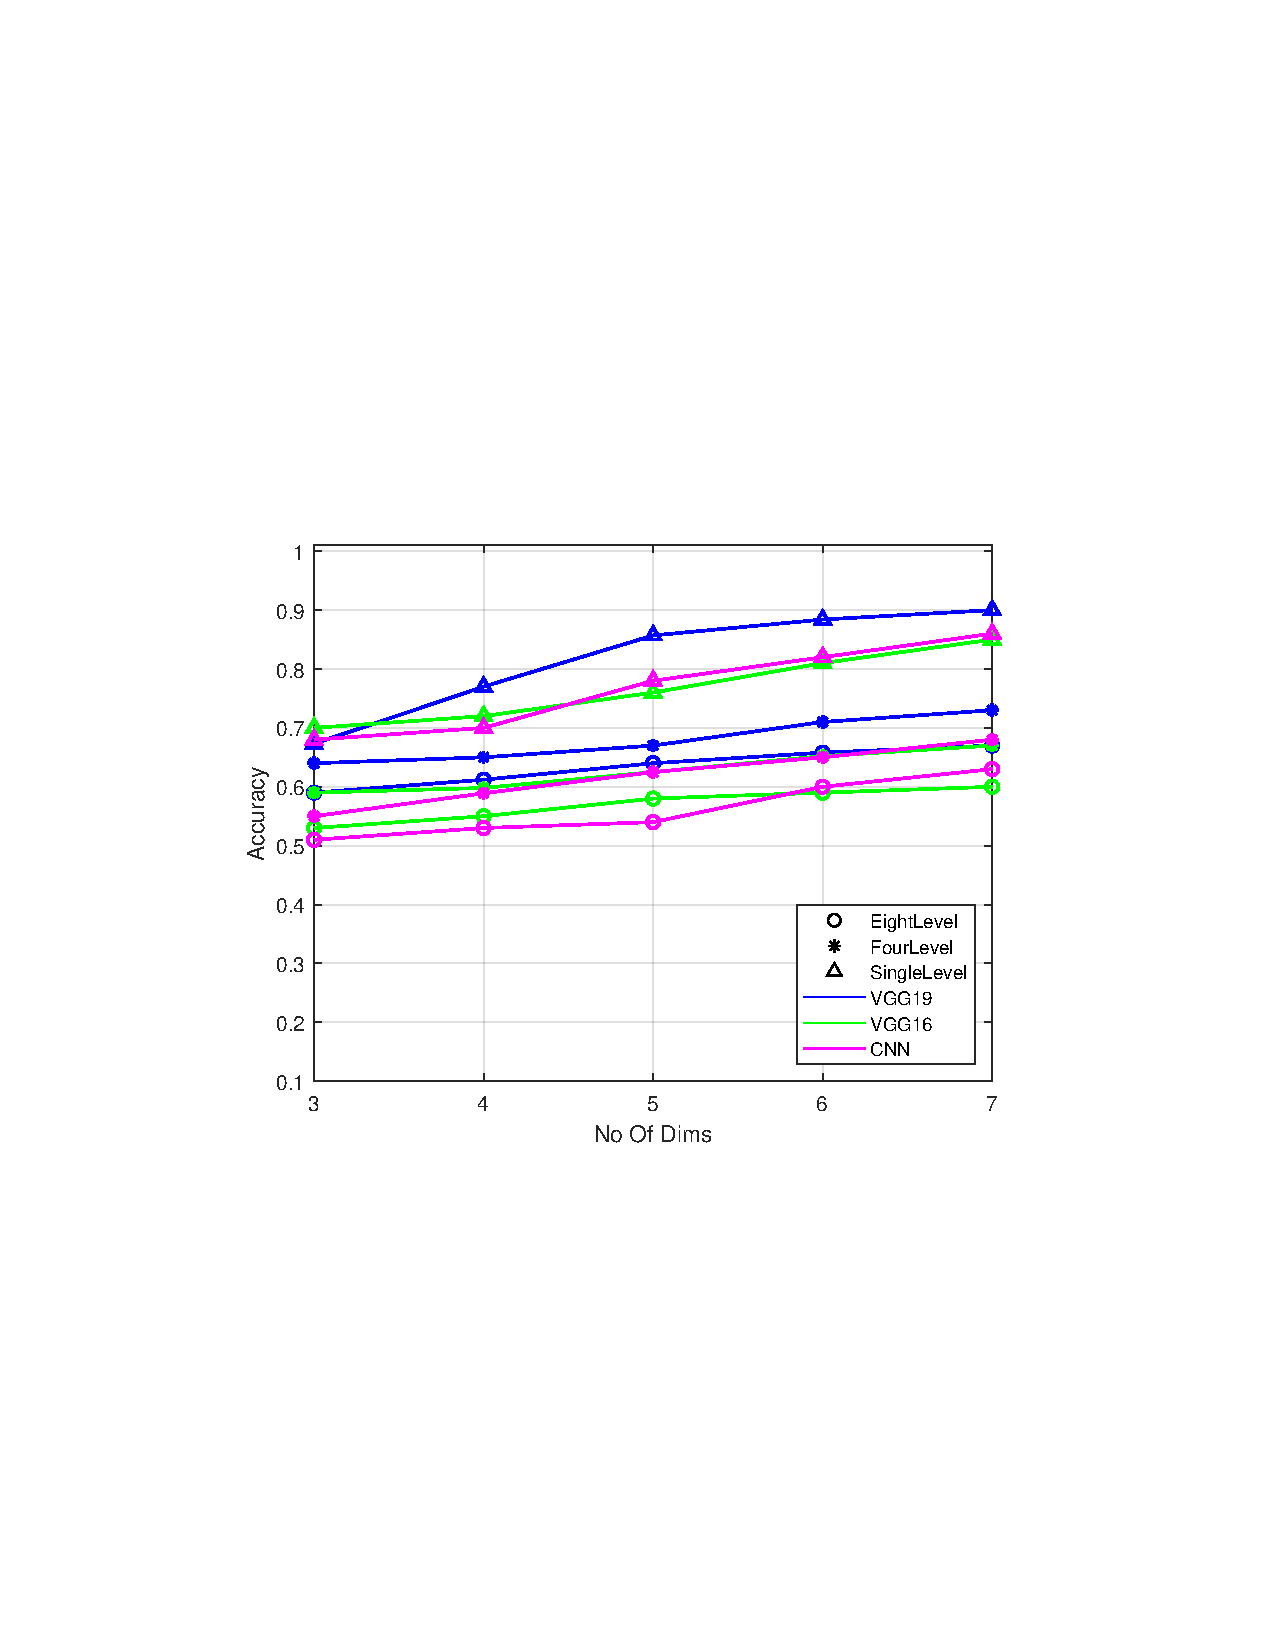
\includegraphics[width=\linewidth, trim=3.8cm 8cm 4cm 8cm, clip=true]{figures/yale_acc}
		\captionsetup{justification=centering}
		\caption{Yale\_B}
		\label{fig:yale_acc}
	\end{subfigure}
	\begin{subfigure}{.33\textwidth}
		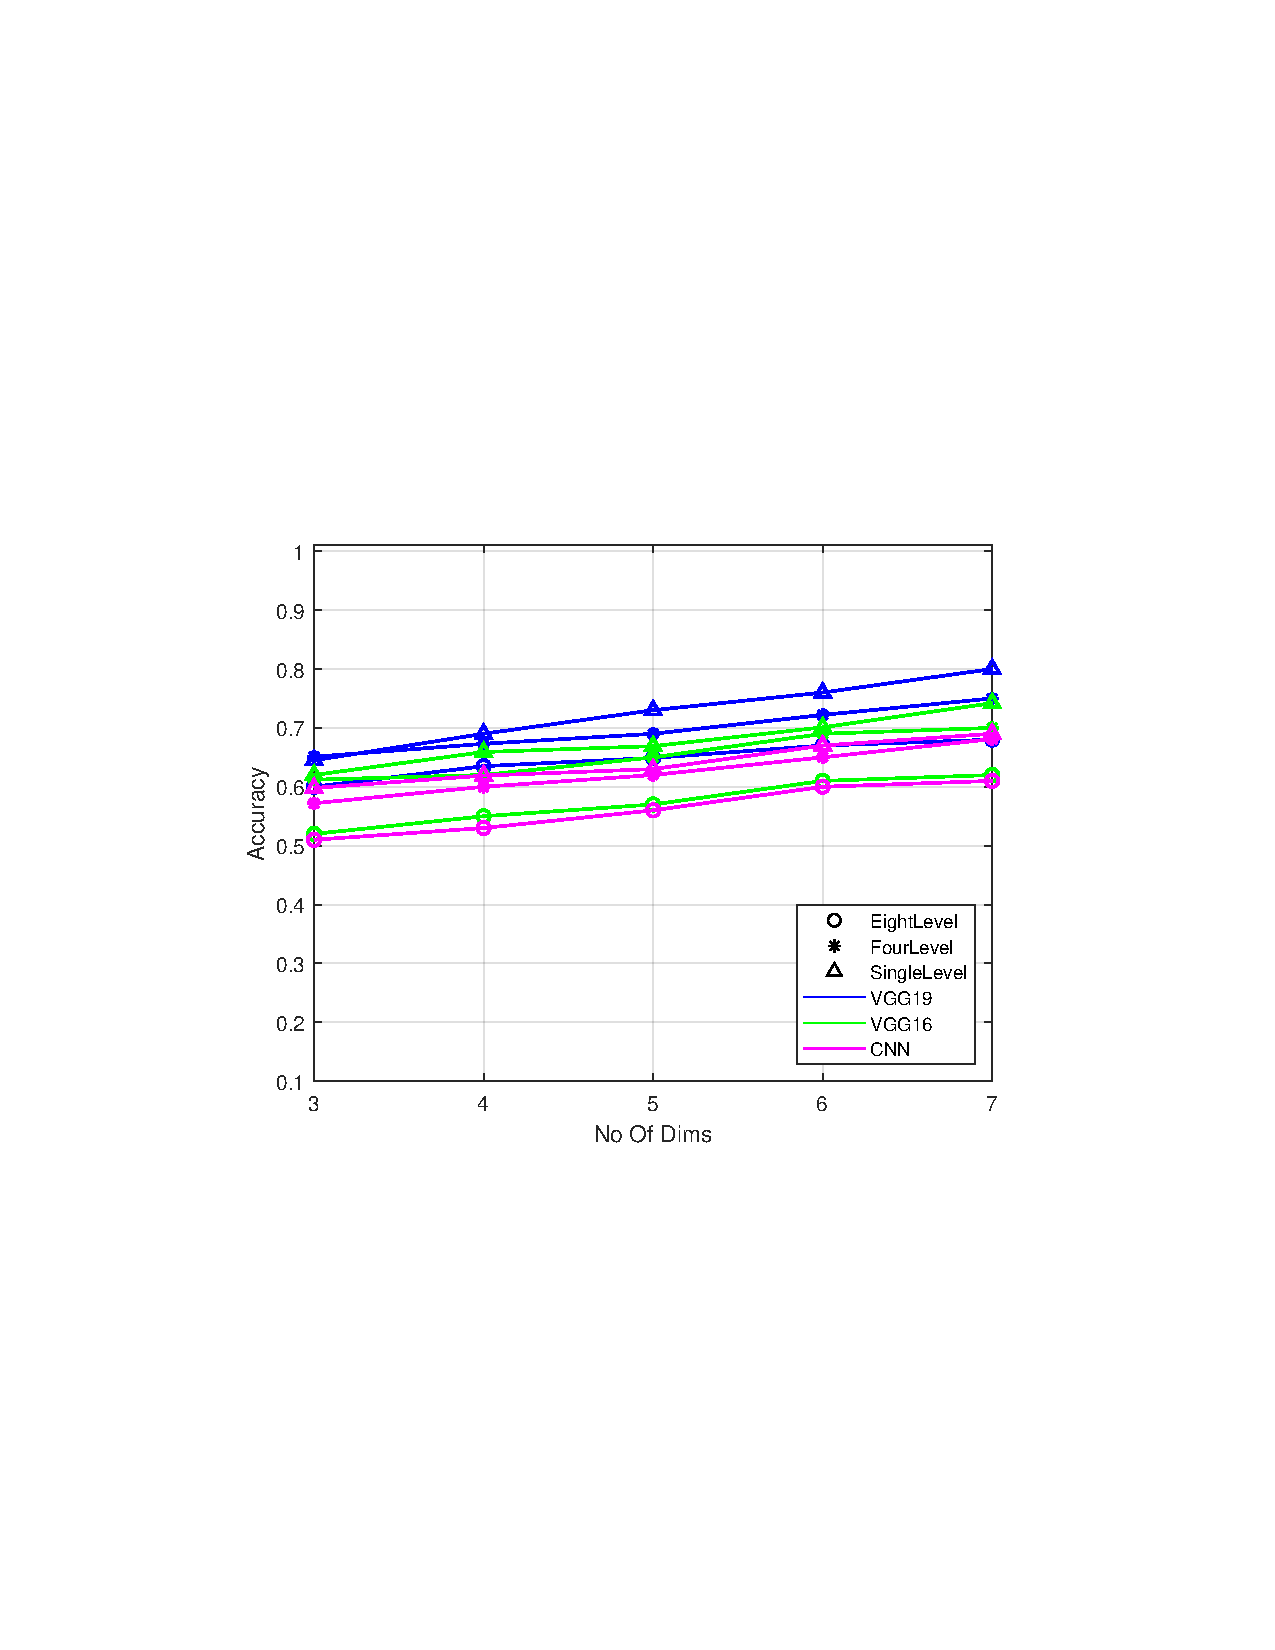
\includegraphics[width=\linewidth, trim=3.8cm 8cm 4cm 8cm, clip=true]{figures/celeba_acc}
		\captionsetup{justification=centering}
		\caption{CelebA}
		\label{fig:celeba_acc}
	\end{subfigure}
	\caption{Accuracy for Different Number of Reduced Dimensions }
	\label{fig:acc}
\end{figure*}

\begin{figure*}[ht!]
	\begin{subfigure}{.33\textwidth}
		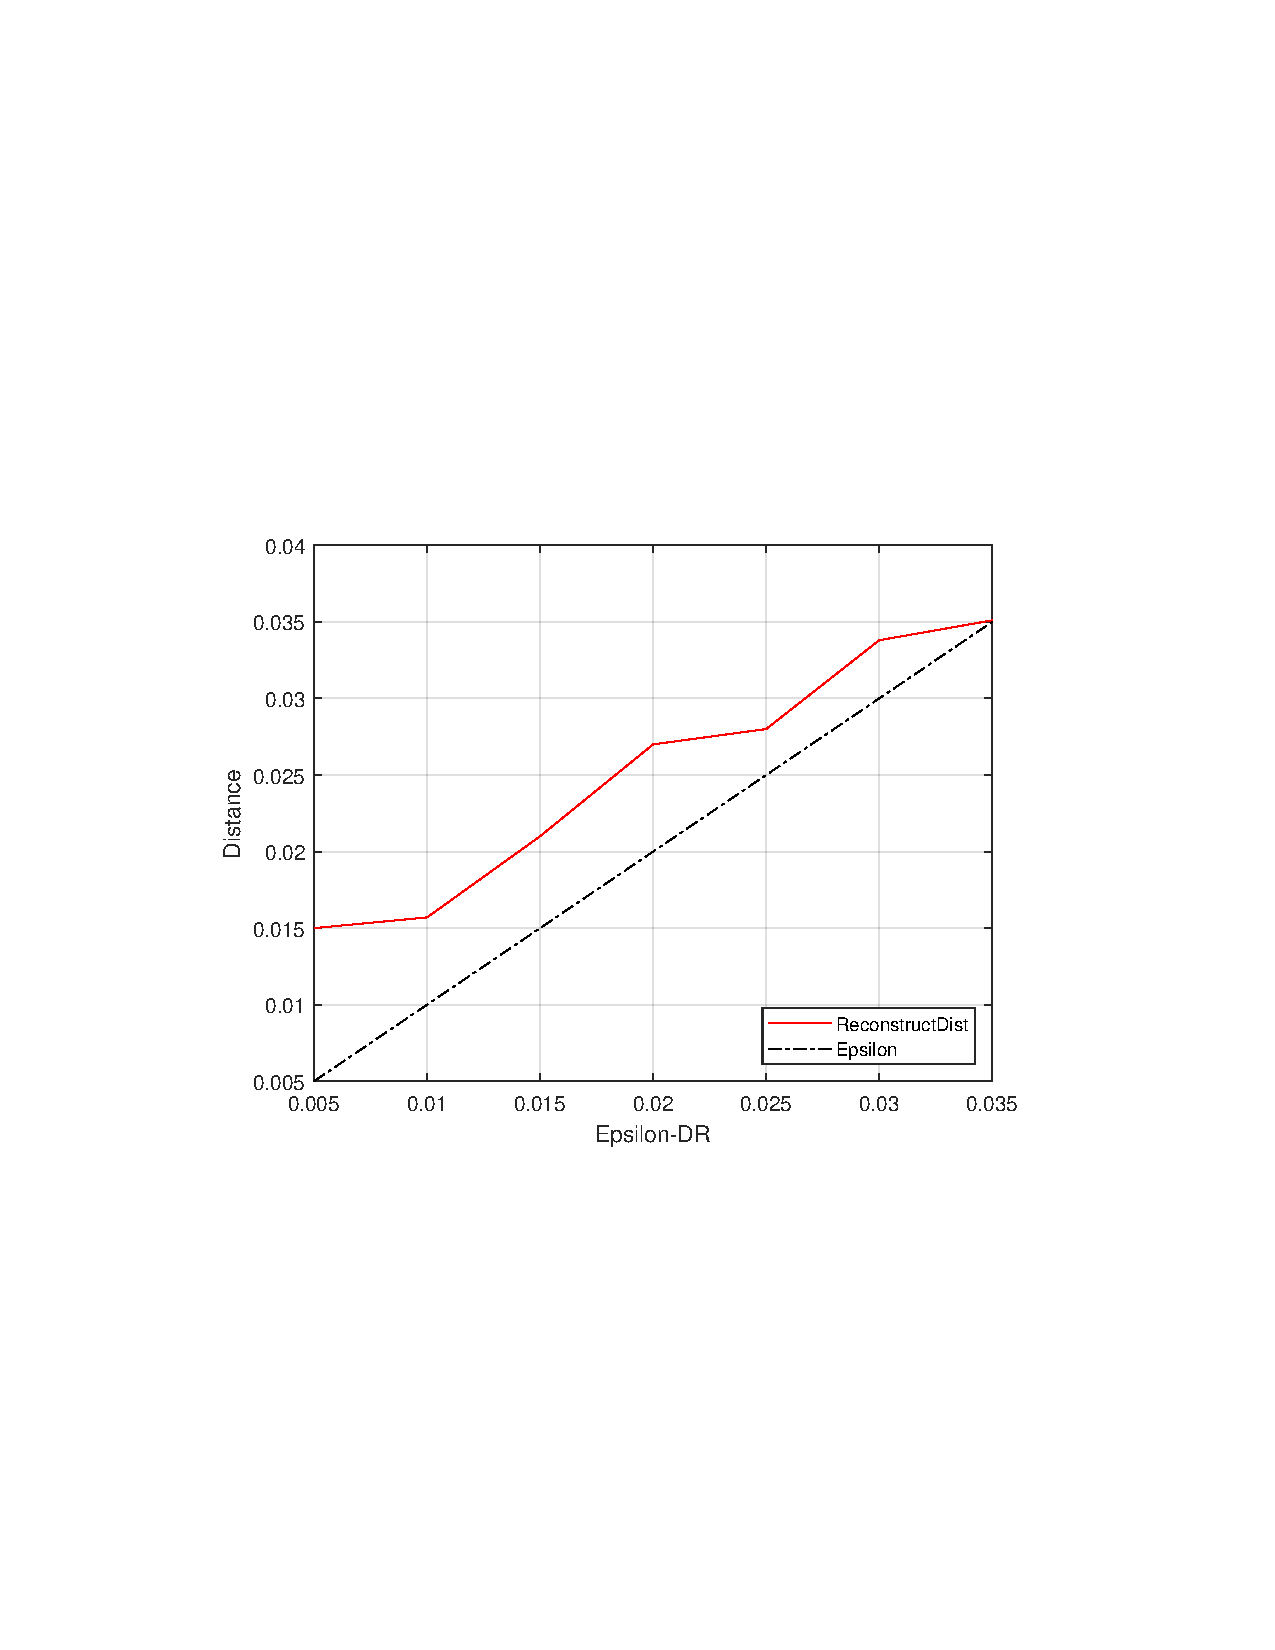
\includegraphics[width=\linewidth, trim=3.8cm 8cm 4cm 8cm, clip=true]{figures/ep_att}
		\captionsetup{justification=centering}
		\caption{ AT\&T}
		\label{fig:att_dist}
	\end{subfigure}
	\begin{subfigure}{.33\textwidth}
		\includegraphics[width=\linewidth, trim=3.8cm 8cm 4cm 8cm, clip=true]{figures/ep_yale}
		\captionsetup{justification=centering}
		\caption{Yale\_B}
		\label{fig:yale_dist}
	\end{subfigure}
	\begin{subfigure}{.33\textwidth}
		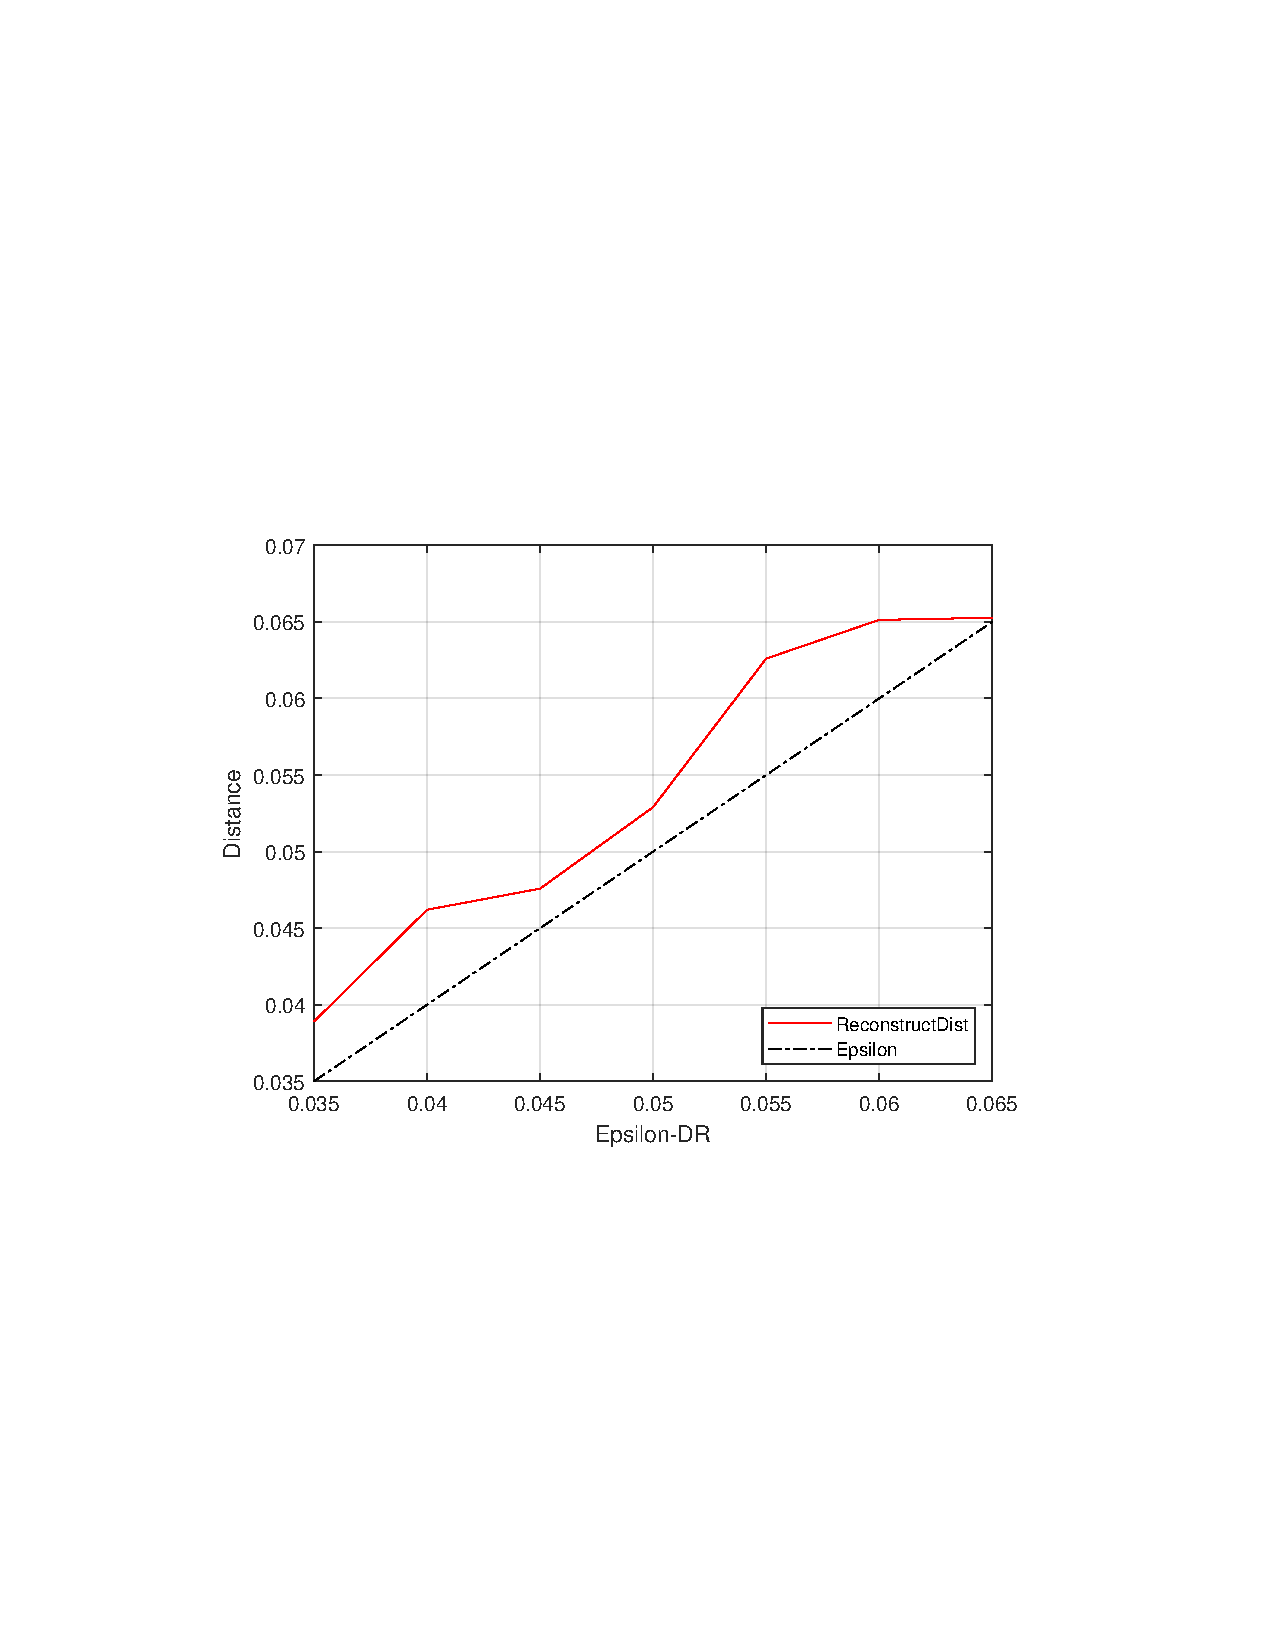
\includegraphics[width=\linewidth, trim=3.8cm 8cm 4cm 8cm, clip=true]{figures/ep_celeba}
		\captionsetup{justification=centering}
		\caption{CelebA}
		\label{fig:celeba_dist}
	\end{subfigure}
	\caption{Average Distance Measurement Result \{ 7 dimensions, Single-Level\}}
	\label{fig:distresult}
\end{figure*}
"


\setcounter{section}{5} "
\section{Visual Comparison to Privacy Preserving Techniques }
\label{AutoGAN_DP_PCA}

In this section, we compare AutoGAN-DRP with other privacy preserving methods in terms of ability to visually identify client's identities. We choose the widely used tool for privacy preserving Differential Privacy (DP) [27] and another privacy preservation method utilizing dimensionality reduction technique (i.e., Principle Component Analysis [34] ).

In these experiments, we implement AutoGAN-DRP following VGG19 structure for the Generator and Re-constructor, and other setting parameters (e.g., number of hidden layers, learning rate, optimization) are shown in Table \ref{table:implementation}. The images are reduced to seven dimensions for different values of $\epsilon$-DR to achieve different distances and accuracies. The datasets are grouped into two groups corresponding to a binary classifier. 

For implementing DP, we first generate a classifier on the authentication server by training the datasets with a VGG19 binary classifier (the structure of hidden layers is similar to our Generator in Table \ref{table:implementation}). The testing images are then perturbed using differential privacy method. Specifically, Laplace noise is added to the images with the sensitivity coefficient of 1 (it is computed by the maximum range value of each pixel [0,1]) and different DP epsilon parameters (this DP epsilon is different from our $\epsilon$-DR). The perturbed images are then sent to the authentication server and fed to the classifier. We visually compare the perturbed images of this method with AutoGAN. 

In addition, we follow instruction in FRiPAL [11] in which the clients reduce image dimension using Principle Component Analysis (PCA) and send reduced features to the server. FRiPAL claims that by reducing image dimension, their method can be more resilient to reconstruction attacks. The experiments are conducted with different number of reduced dimension. The images are reconstructed using \textit{Moore–Penrose inverse} method with assumption that an adversary has assess to the model. The classification accuracy is evaluated using a classifier which has similar structure to AutoGAN's classifier. 

Table \ref{table:visualization} shows image samples and results over the three datasets. Overall, AutoGAN-DRP is more resilient to reconstruction attacks compared to the other two techniques. For instance, at the accuracy of 79\% on AT\&T dataset, 80\% on YaleB, and 73\% on CelebA, we cannot distinguish entities from the others. For DP method, the accuracy decreases when the DP epsilon decreases (adding more noise), and the perturbed images become harder to recognize. However, at a low accuracy 57\%, we are still able to distinguish identities by human eyes. The reason is that DP noise does not focus on the important visual pixels. For PCA, the accuracy also goes down when the number of dimensions decreases and the distances increase. Since PCA transformation is linear and deterministic, the original information can be significantly reconstructed using the inverse transformation deriving from the model or training data. Thus, at the accuracy of 75\% on AT\&T, 71\% on YaleB, and 68\% on CelebA, we still can differentiate individuals. Overall, our proposed method shows the advantage in securing the data while retaining high data utility.       
\\ 
\setcounter{table}{1}

\begin{table}[H]
	\centering
	%trim  left, bottom, right and top 
	\includegraphics[width=0.8\linewidth, trim=1cm 3cm 1cm 3cm, clip=true]{tables/img_table}
	\caption{Sample visualization of AutoGAN, DP, PCA over three datasets}
	\label{table:visualization}
\end{table}

"

\color{blue}
\underline{Comment 2.7}
What is the advantage of AutoGAN-DRP in terms of privacy protection compared to GAP?  The advice I would like to give is that the authors could give more details to explain the advantages of this method further. 

\color{black}
\underline{Response:}

AutoGAN-DRP is visually protecting the images themselves by reducing image dimension and extracting the most important information of images which maintains utility of data. As shown in Figure \ref{fig:genki}, at the same distortion level AutoGAN provides higher accuracy which implies our method can add more noise than GAP but still maintain high data utility. 

\setcounter{figure}{6} 
\begin{figure}[H]
	\centering
	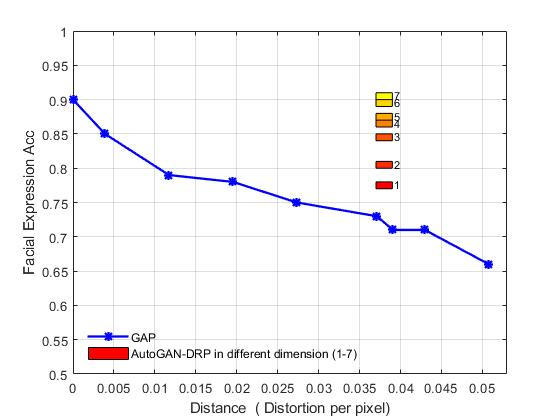
\includegraphics[width=.6\linewidth]{supplement/comparison_GAP/ACC_AutoGANvsGAP}
	\captionsetup{justification=centering}
	\caption{GENKI Facial Expression Accuracy Vs Distance using GAP and AutoGAN-DRP}
	\label{fig:genki}
\end{figure}

To provide readers intuitive information about our method privacy preservation capacity, we conducted more comparison experiments as presented in Section 6 Visual comparison to privacy preservation techniques using Differential Privacy (DP) [24] and Principle Component Analysis (PCA) [33] as follows.


	\setcounter{section}{5} "
	\section{Visual comparison to privacy preservation techniques using Differential Privacy (DP) [27] and Principle Component Analysis (PCA) [33]}
	\label{AutoGAN_DP_PCA}
	In this section, we compare AutoGAN-DRP with other privacy preserving methods in terms of ability to visually identify client's identities. We choose the widely used tool for privacy preserving Differential Privacy (DP) [27] and another privacy preservation method utilizing dimensionality reduction technique (i.e., Principle Component Analysis [34] ).
	
	In these experiments, we implement AutoGAN-DRP following VGG19 structure for the Generator and Re-constructor, and other setting parameters (e.g., number of hidden layers, learning rate, optimization) are shown in Table \ref{table:implementation}. The images are reduced to seven dimensions for different values of $\epsilon$-DR to achieve different distances and accuracies. The datasets are grouped into two groups corresponding to a binary classifier. 
	
	For implementing DP, we first generate a classifier on the authentication server by training the datasets with a VGG19 binary classifier (the structure of hidden layers is similar to our Generator in Table \ref{table:implementation}). The testing images are then perturbed using differential privacy method. Specifically, Laplace noise is added to the images with the sensitivity coefficient of 1 (it is computed by the maximum range value of each pixel [0,1]) and different DP epsilon parameters (this DP epsilon is different from our $\epsilon$-DR). The perturbed images are then sent to the authentication server and fed to the classifier. We visually compare the perturbed images of this method with AutoGAN. 
	
	In addition, we follow instruction in FRiPAL [11] in which the clients reduce image dimension using Principle Component Analysis (PCA) and send reduced features to the server. FRiPAL claims that by reducing image dimension, their method can be more resilient to reconstruction attacks. The experiments are conducted with different number of reduced dimension. The images are reconstructed using \textit{Moore–Penrose inverse} method with assumption that an adversary has assess to the model. The classification accuracy is evaluated using a classifier which has similar structure to AutoGAN's classifier.  
	
	Table \ref{table:visualization} shows image samples and results over the three datasets. Overall, AutoGAN-DRP is more resilient to reconstruction attacks compared to the other two techniques. For instance, at the accuracy of 79\% on AT\&T dataset, 80\% on YaleB, and 73\% on CelebA, we cannot distinguish entities from the others. For DP method, the accuracy decreases when the DP epsilon decreases (adding more noise), and the perturbed images become harder to recognize. However, at a low accuracy 57\%, we are still able to distinguish identities by human eyes. The reason is that DP noise does not focus on the important visual pixels. For PCA, the accuracy also goes down when the number of dimensions decreases and the distances increase. Since PCA transformation is linear and deterministic, the original information can be significantly reconstructed using the inverse transformation deriving from the model or training data. Thus, at the accuracy of 75\% on AT\&T, 71\% on YaleB, and 68\% on CelebA, we still can differentiate individuals. Overall, our proposed method shows the advantage in securing the data while retaining high data utility.  "
	\\ 
	\setcounter{table}{1}
	\begin{table}[H]
		\centering
		%trim  left, bottom, right and top 
		\includegraphics[width=0.8\linewidth, trim=1cm 3cm 1cm 3cm, clip=true]{supplement/image_table/img_table}
		\caption{Sample visualization of AutoGAN, DP, PCA over three datasets}
		\label{table:visualization}
	\end{table}  



\color{blue}
\underline{Comment 2.8}
Please rearrange the chart in paper, I hope it can help the paper to improve the readability. 
	
\color{black}
\underline{Response:}

Thank you for your suggestion. In this revision, we rearranged figures and tables by putting them closed to their related sections.\\


 
\color{blue}
\underline{Comment 2.9}
In Section 6.2, there is a spelling mistake, please correct it. 

\color{black}
\underline{Response:}


Thank you for your comment. In this revision, we fixed that spelling mistake\\. 



\color{blue}
\underline{Comment 2.10}
In the paper, some formulas have no serial numbers, please correct it. 

\color{black}
\underline{Response:}


Thank you for your comment. In this revision, we added serial numbers on all of the formulas.\\


\color{blue}
\underline{Comment 2.11}  
The number of references is insufficient, please add the corresponding references, I hope this will help to improve the quality of the paper.

\color{black}
\underline{Response:}

Thank you for the comment. According to your recommendation, we updated our references
for the most recent years in the related work (10 references added). \\



\newpage
\begin{enumerate}[III.]
	\item RESPONSE TO REVIEWER 3
\end{enumerate}
\color{blue}
Overall, this paper proposed a GAN-based dimension reduction method for privacy preservation. The motivation is practical while the method is well presented. However the novelty is still limited and the authors need to explain more clearer about their contribution.

\underline{Comment 3.1}
The main optimization formulation needs more explanation, especially from the perspective of theoretical analysis.

\color{black}
\underline{Response:}


Thank you for the comment. In this revision, we revised to clarify the main optimization and updated Section 3.3 (AutoGAN-based Dimension Reduction for Privacy Preserving) to give more explanation as follows.


	"\dots
	Our proposed framework is designed to learn a DR function $F(\cdot)$ that projects data onto low dimension space and preserves privacy at certain value of $\epsilon$. The larger distance implies higher level of privacy. Figure \ref{fig:eGAN} presents our learning system in which the dimension-reduced data $X'$ is given by a generator $G$. Since $X'$ is expected to be accurately classified by a classifier $C$, the generator improves by receiving feedback from the classifier via the classifier's loss function $\mathcal{L}_C$. We use a binary classifier for single-level authentication system and multi-class classifiers for multi-level authentication system. The classifier loss function is defined as the cross entropy loss of the ground truth label $y$ and predicted label $\hat y$ as follows.
	
	\begin{equation}
	\mathcal{L}_C=-\sum_{i=1}^n\sum_{j=1}^m y_{ij} \log(\hat y_{ij})  
	%\quad y,\hat y \in \{0,1,..,m-1\}
	\label{C_loss}
	\end{equation}
	where $m$ denotes the number of classes and $n$ denotes the number of samples.
	
	To evaluate data reconstruction and enlarge the reconstruction distance, a re-constructor $R$ is trained as a decoder in an auto-encoder and sends feedback to the generator via its loss function $\mathcal{L}_R$. The re-constructor plays its role as an aggressive adversary attempting to reconstruct original data by using known data. The loss function of $R$ is the mean square error of original training data ($x$) and reconstructed data ($\hat x$), as displayed in (\ref{R_loss}).
	\begin{align}
	\mathcal{L}_R = \sum_{i=1}^n{(x_i - \hat x_i)^2} 
	\label{R_loss}
	\end{align}   
	
	To direct the reconstructed data to a direction that reveals less visual information, the generator is trained with a discriminator $D$ as a minimax game in GAN. The motivation is to direct reconstructed data to a certain target distribution (e.g., normal distribution). To ensure a distance, the target distribution should be different to training data distribution. The discriminator aims to differentiate the reconstructed data from samples of the target distribution. The loss function of $D$ ($\mathcal{L}_D$) can be defined as a cross-entropy loss of ground truth labels (0 or 1) $t$ and prediction labels $\hat t$ shown in (\ref{D_loss}).
	
	\begin{equation}
	\mathcal{L}_D = -\sum_{i=1}^n{(t_i\log(\hat t_i) + (1 - t_i)\log(1 - \hat t_i))} 
	\label{D_loss}
	\end{equation}
	
	The optimal generator parameter $\theta^*$ is given by the optimization problem of the generator loss function  $\mathcal{L}_G$:
	\begin{equation}
	\underset{\theta}{minimize} \; \mathcal{L}_G(\theta) = \alpha \min\limits_{\phi}{\mathcal{L}_C} - \beta\min\limits_{\omega}{\mathcal{L}_D}
	-\gamma\min\limits_{\varphi}{\mathcal{L}_R} + \mathcal{C}(\epsilon)
	\label{eqn:G_loss}
	\end{equation}  
	where $\theta$, $\phi$, $\omega$, and $\varphi$ are the model parameters of the generator, classifier, discriminator, and re-constructor respectively. $\alpha$, $\beta$, and $\gamma$ are weights of components in the objective function of the generator and can be freely tuned. $\mathcal{C}(\epsilon)$ is a constraint function with respect to hyper-parameter $\epsilon$, as to be elaborated in the following subsection.
	
	\subsection{Optimization With Constraint}
	In order to meet a certain level of reconstruction distance, we consider the constrained problem:
	
	\begin{equation}
	\begin{array}{l}
	\; \; \; \;\underset{\theta}{minimize} \;\mathcal{L}_G(\theta) \\ 
	s.t \; \; \;  \mathbb{E}_{x \sim p_d}[dist(x, \hat{x})] \leq \epsilon  
	\end{array}
	\label{constr}
	\end{equation}
	
	The optimization problem above can be approximated as an unconstrained problem [32]:
	\begin{equation} 
	\underset{\theta}{minimize} \; ( \mathcal{L}_G(\theta) + \gamma \mathcal{C}(\epsilon) )  
	\end{equation}
	where $\gamma$ is a penalty parameter and $\mathcal{C}$ is a penalty function 
	
	\begin{equation} 
	\mathcal{C}(\epsilon) = \max(0, \mathbb{E}_{x \sim p_d}[dist(x, \hat{x})] -\epsilon)
	\end{equation}
	Note that $\mathcal{C}$ is nonnegative, and $\mathcal{C}(\theta)=0$ iff the constraint in (\ref{constr}) is satisfied.
	\setcounter{figure}{2}
	\begin{figure}[H]
		\centering
		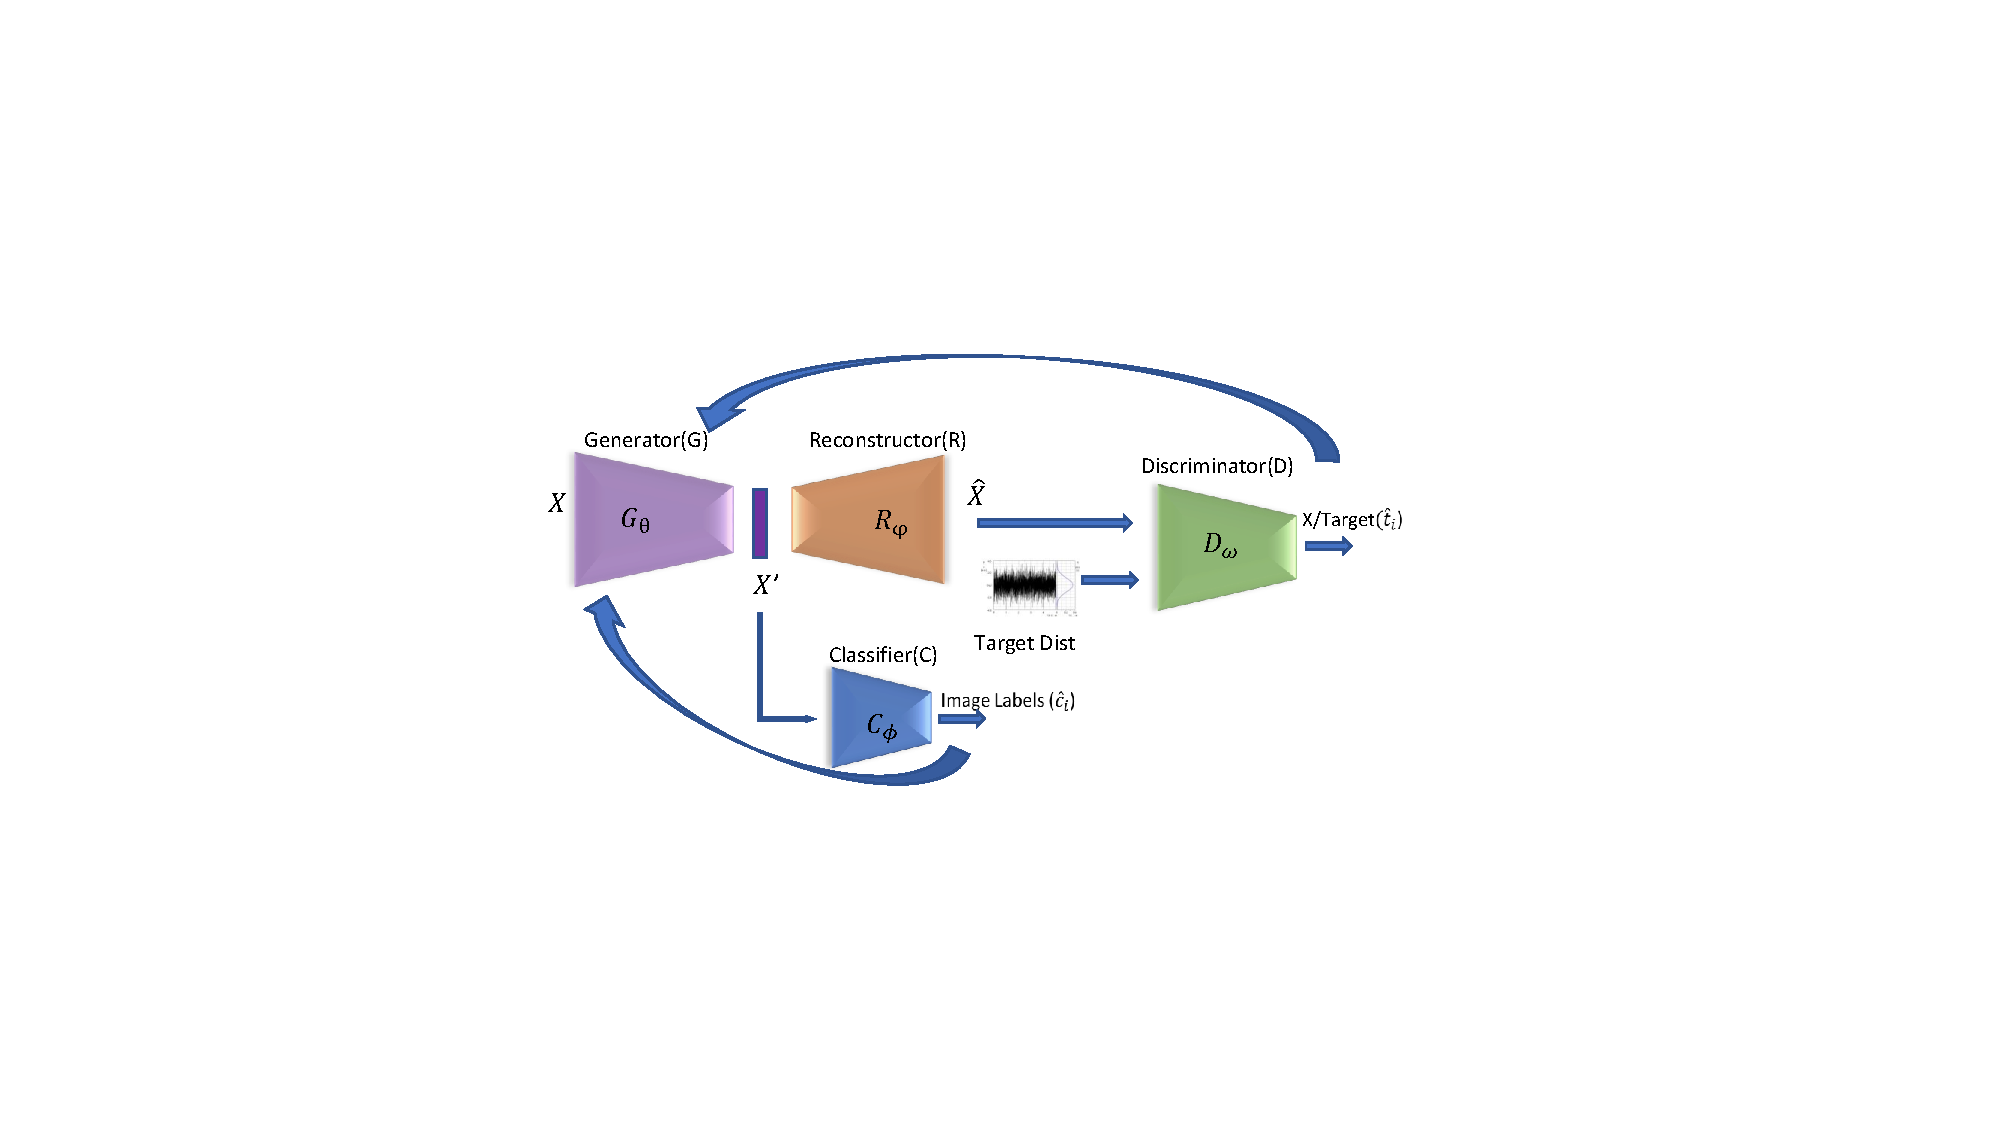
\includegraphics[width=1\linewidth]{figures/eGAN}
		\captionsetup{justification=centering}
		\caption{AutoGAN-DRP}
		\label{fig:eGAN}
	\end{figure}
	"  




\color{blue}
\underline{Comment 3.2} 
Not enough comparison in the experiments section, especially evaluation standard is not clear

\color{black}
\underline{Response:}


Thank you for your comments. To provide more comparison information, in this revision, we conducted more experiments using most current powerful structure of convolution networks (i.e., VGG16, VGG19 [32], basic CNN) for the Generator and their inverted structures for the Re-constructor (Section 4 was updated accordingly). By examining most recent powerful structures of re-constructors, we aim at evaluating strong adversaries who attempt to reconstruct our original data. Beside the comparison with GAP in Section 5, we also conduct more experiments (Section 6 was added) to compare with other privacy preservation techniques (i.e., Differential Privacy, Principle Component Analysis for privacy preservation).

Regarding evaluation standard, we evaluated data utility by examining the classification accuracy. Higher accuracy is considered as more utility was preserved. For privacy, we consider the reconstruction distance between the reconstructed images and the original images. Larger distance is better. we also look at the visualization of reconstructed images as another privacy preserving aspect. The reconstruction distance in this case is defined as L\_2 norm distance. In this revision, we clarify this in Section 4.3 (Privacy) as follows.

"
In this study, the Euclidean distance is used to measure the distance between original and reconstructed images: $dist(x,\hat{x}) = ||x-\hat{x}||^2$. 
" 

we updated more experiments in Section 4 (Experiment and Discussion) and added one more comparison section (Section 6) as follows.\\


\titleformat*{\subsection}{\normalsize\itshape}
\titleformat*{\section}{\normalsize\itshape}
\setcounter{section}{3}"
\section{Experiments and Discussion}
In this section, we demonstrate our experiments over three popular supervised face image datasets: \textit{the Extended Yale Face Database B} [18], \textit{AT}\&\textit{T} [19], and \textit{CelebFaces Attributes Dataset (CelebA)} [20]. To evaluate our method performance, we also conduct experiments with different generator and re-constructor structures, different types of classifications (binary and multi-class classification), different numbers of reduced dimensions. The effectiveness of the method is then evaluated in terms of utility and privacy.   
\subsection{Experiment Setup}
\textit{The Extended Yale Face Database B} (YaleB) contains 2,470 grayscale images of 38 human subjects under different illumination conditions and their identity label. In this dataset, the image size is 168$\times$192 pixels. The AT\&T dataset has 400 face images of 40 subjects. For convenience, we resize each image of these two dataset to 64$\times$64 pixels. CelebA is a color facial image dataset containing 202,599 images of 10,177 subjects. 1,709 images of the first 80 subjects are used for our experiment. Each image is resized to 64$\times$64$\times$3 pixels. All pixel values are scaled to the range of [0,1]. We randomly select 10\% of each subject's images for validation and 15\% for testing dataset. 

The generator and re-constructor in Figure \ref{fig:eGAN} are implemented by three different structures. Specifically, we follow the architecture of recent powerful models VGG19, VGG16 [33] and a basic convolutional network (CNN). We modify the models to adapt to our data size (64$\times$64). Discriminator and Classifier are built on fully connected neural network and convolutional network respectively. Leaky ReLU is used for activation function in hidden layers. We use linear activation function for generator's output layers and softmax activation functions for other components' output layers. Each component is trained in 5 local iterations ($n_r, n_g, n_d, n_c$), and the entire system is trained in 500 global iterations ($n$). The target distribution is drawn from Gaussian distribution (with the covariance value of 0.5 and the mean is the average of the training data). Table \ref{table:implementation} provides detail information of neural networks' structures and other implementation information. 

\setcounter{table}{0}
\begin{table}[H]
	\centering
	%trim  left, bottom, right and top 
	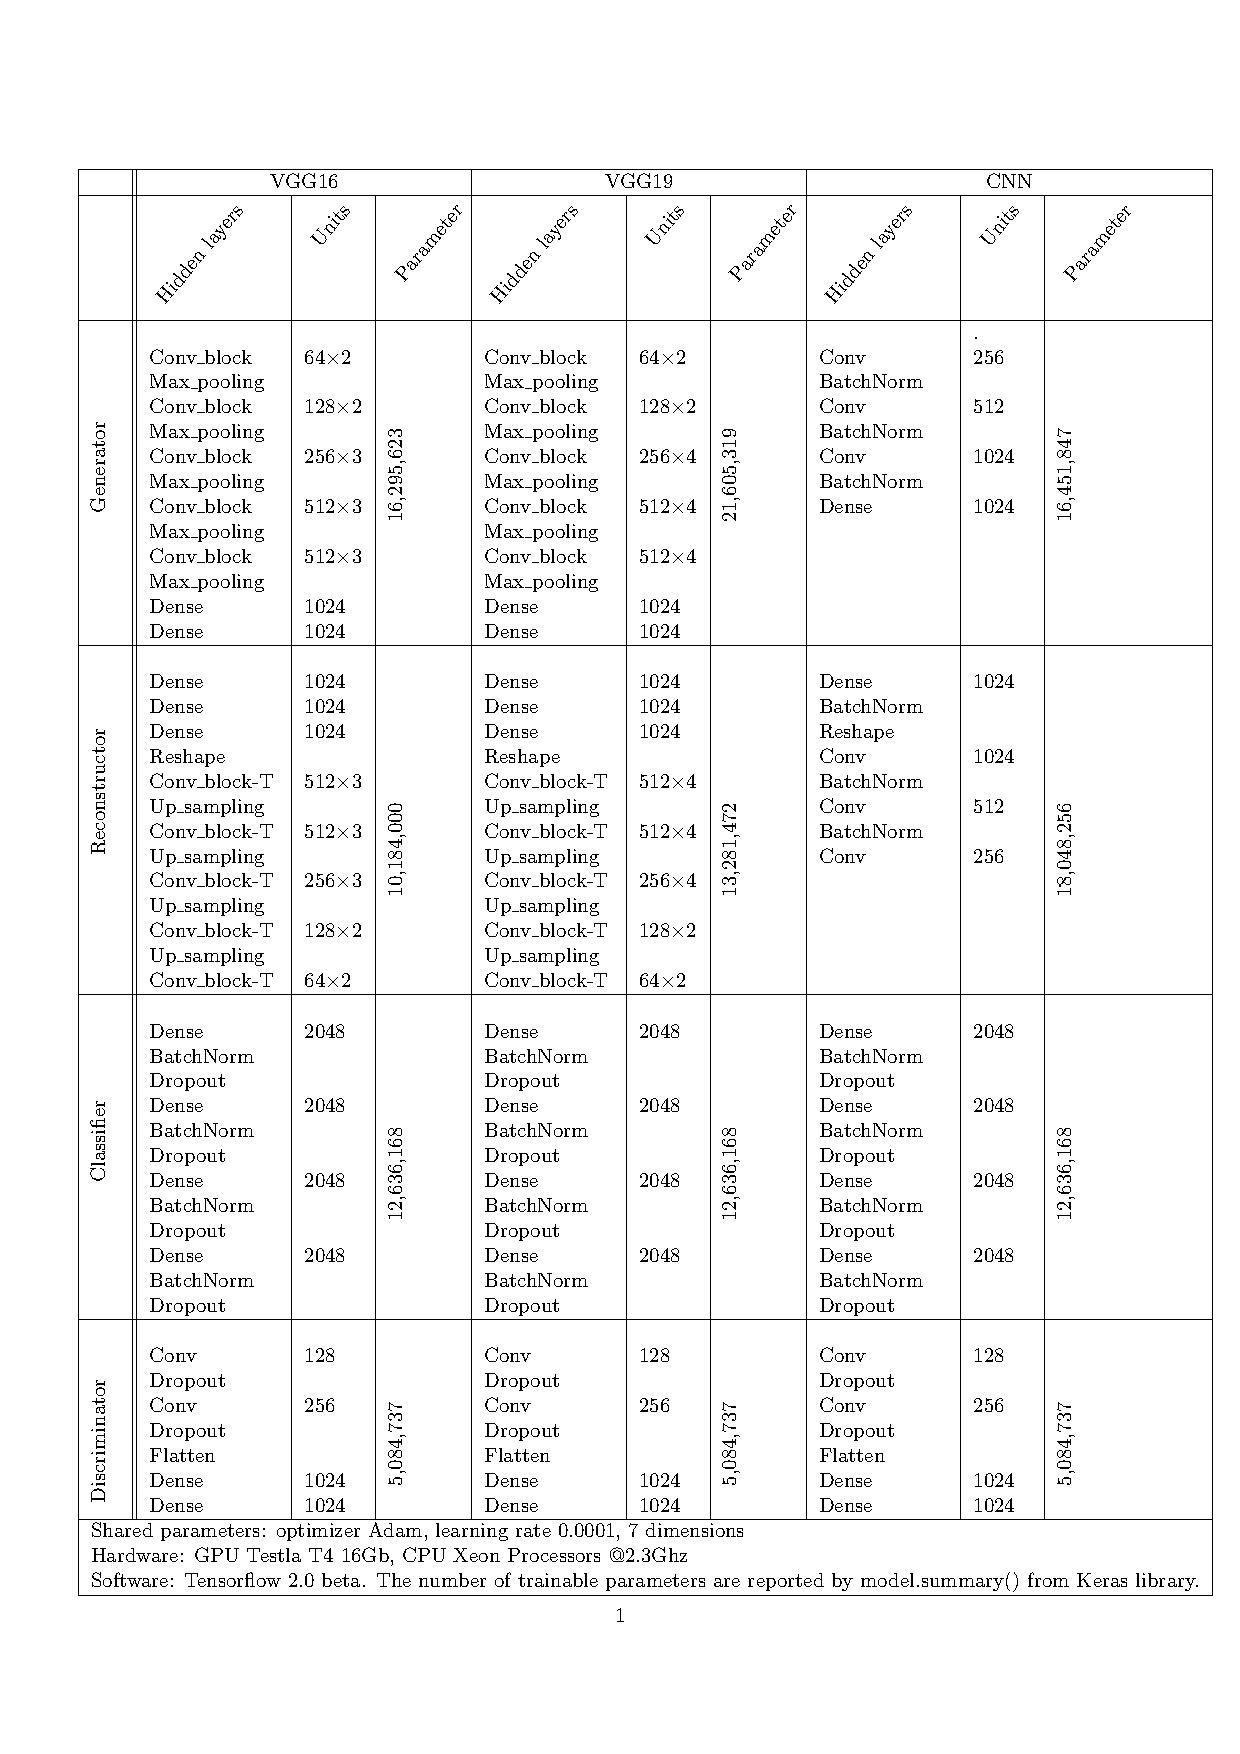
\includegraphics[width=0.7\linewidth, trim=1cm 2.5cm 0.1cm 2.5cm, clip=true]{tables/implement_table}
	\caption{Implementation information}
	\label{table:implementation}
\end{table}

To evaluate the reliability, we test our framework with different levels of authentication corresponding to binary classification (single-level) and multi-class classification (multi-level). For the single-level authentication system, we consider half of the subjects in the dataset are valid to access company's resources while the rest are invalid. We randomly divide the dataset into two groups of subjects and labels their images to (1) or (0) depending on their access permission. For the cases of multi-level authentication system, we divide the subjects into four groups and eight groups. Therefore, the authentication server becomes four-class and eight-class classifier respectively. 
\subsection{Utility}
We use accuracy metric to evaluate the utility of dimension-reduced data. The testing dataset is tested with the classifier extracted from our framework. Different structures of Generator and re-constructor are applied including VGG19, VGG16, basic CNN on different privilege levels which correspond to multi-class classification. Figure \ref{fig:acc} illustrates the accuracies for different dimensions from three to seven over the three facial datasets. Overall, the accuracies improve when the number of dimension increases. The accuracies on the two gray image datasets (AT\&T and Yale\_B) reaches 90\% and higher when using VGG with only seven dimensions. This accuracy figure for Celeba is smaller, but it still reaches 80\%. In general, VGG19 structure performs better than using VGG16 and basic CNN in terms of utility due to the complexity (table \ref{table:implementation}) and adaptability to image datasets of VGG19. As the dimension number is reduced from 4,096 (64$\times$64) to 7, we can achieve a compression ratio of 585 yet achieve accuracy of 90\% for the two gray datasets and 80\% for the color dataset. This implies our method could gain a high compression ratio and maintain a high utility in terms of accuracy. During conducting experiments we also observe that the accuracy could be higher if we keep the original resolution of images. However, for convenience and reducing the complexity of our structure, we resize images to the size of 64$\times$64 pixels.    

\subsection{Privacy}
In this study, the Euclidean distance is used to measure the distance between original and reconstructed images: $dist(x,\hat{x}) = ||x-\hat{x}||^2$. Figure \ref{fig:distresult} illustrates the average distances between original images and reconstructed images on testing data with different $\epsilon$ constraints (other setting parameters: seven dimensions, single-level authentication, and VGG19 structure). The achieved distances (red lines) are larger than the hyper-parameter $\epsilon$ (black dotted lines) where $\epsilon$ is less than 0.035 for AT\&T, 0.052 for YaleB and 0.067 for CelebA. Thus, our framework can satisfy $\epsilon$-DR with $\epsilon$ of above values. Due to the fact that the re-constructor obtained some information (we consider the adversary can reach the model and the training data), we can only set the distance constraint $\epsilon$ within a certain range as shown in \ref{fig:distresult}. The intersection between the red line and the dotted black line points out the largest distance our framework can achieve. Since the mean of the target distribution is set to be the same as the mean of training dataset, reconstructed images will be close to the mean of training dataset which we believe it will enlarge the distance and expose less individual information. Thus, the range of epsilon can be estimated base on the expectation of the distance between testing samples and the mean of training data. In addition, the first section of Table \ref{table:visualization} demonstrates some samples and their corresponding reconstructions in single-level authentication and seven dimensions with different achieved accuracies and distances. The reconstructed images could be nearly identical, thus making it visually difficult to recognize the identity of an individual.      
 
\setcounter{figure}{3}	
\begin{figure*}[ht!]
	\begin{subfigure}{.33\textwidth}
		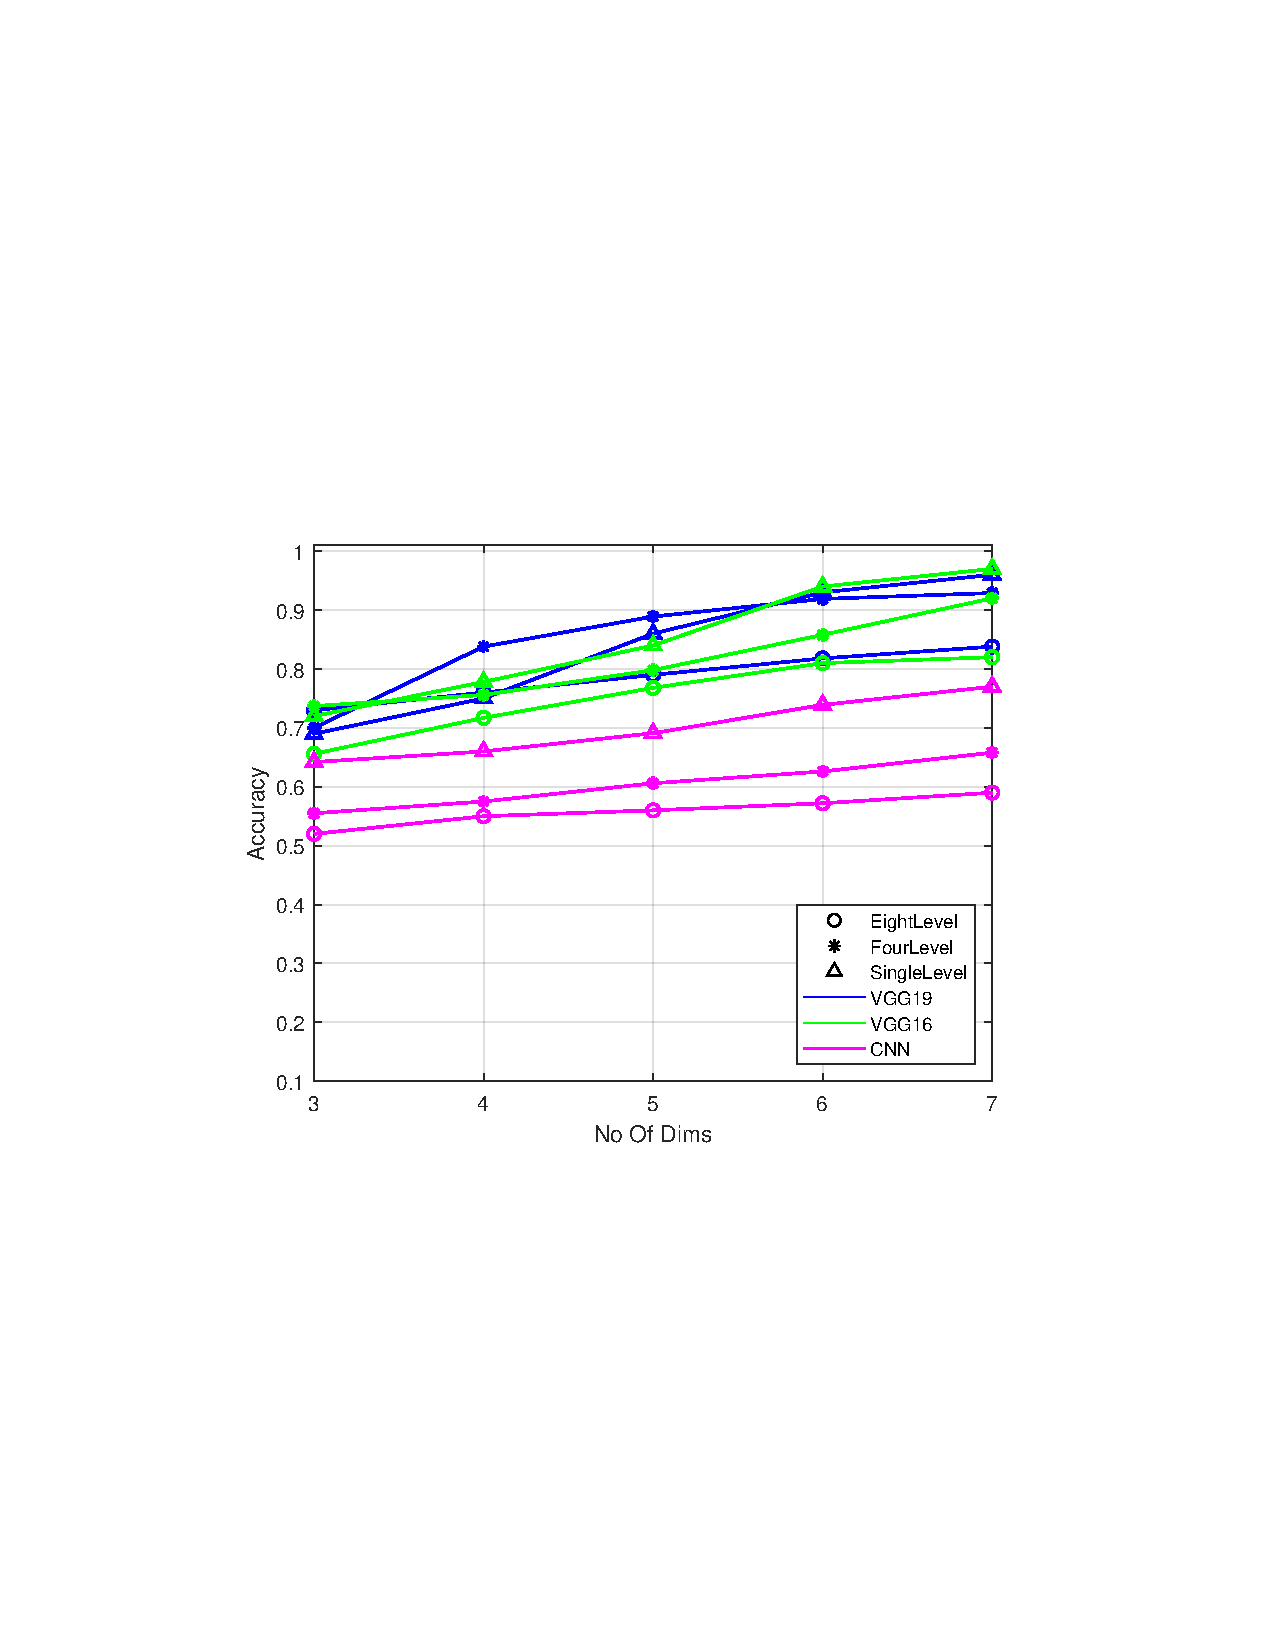
\includegraphics[width=\linewidth, trim=3.8cm 8cm 4cm 8cm, clip=true]{figures/att_acc}
		\captionsetup{justification=centering}
		\caption{ AT\&T}
		\label{fig:att_acc}
	\end{subfigure}
	\begin{subfigure}{.33\textwidth}
		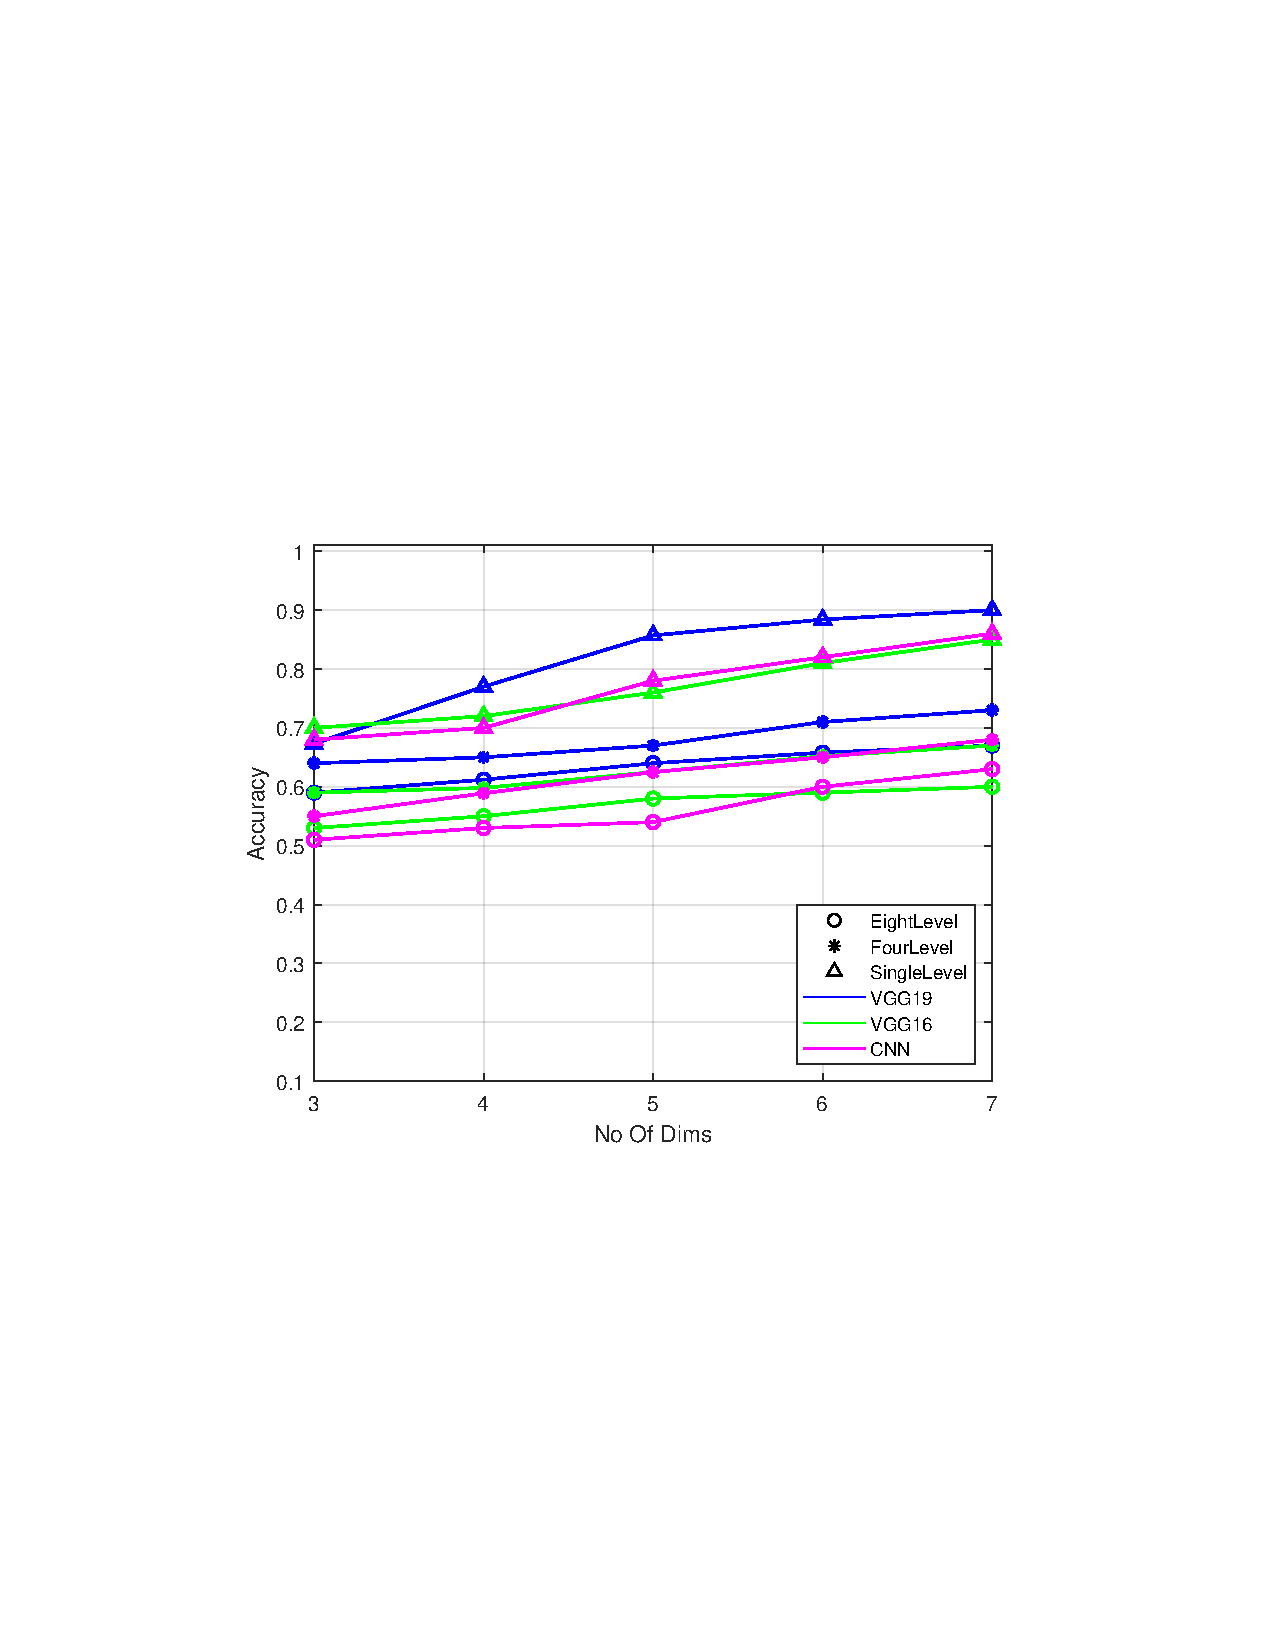
\includegraphics[width=\linewidth, trim=3.8cm 8cm 4cm 8cm, clip=true]{figures/yale_acc}
		\captionsetup{justification=centering}
		\caption{Yale\_B}
		\label{fig:yale_acc}
	\end{subfigure}
	\begin{subfigure}{.33\textwidth}
		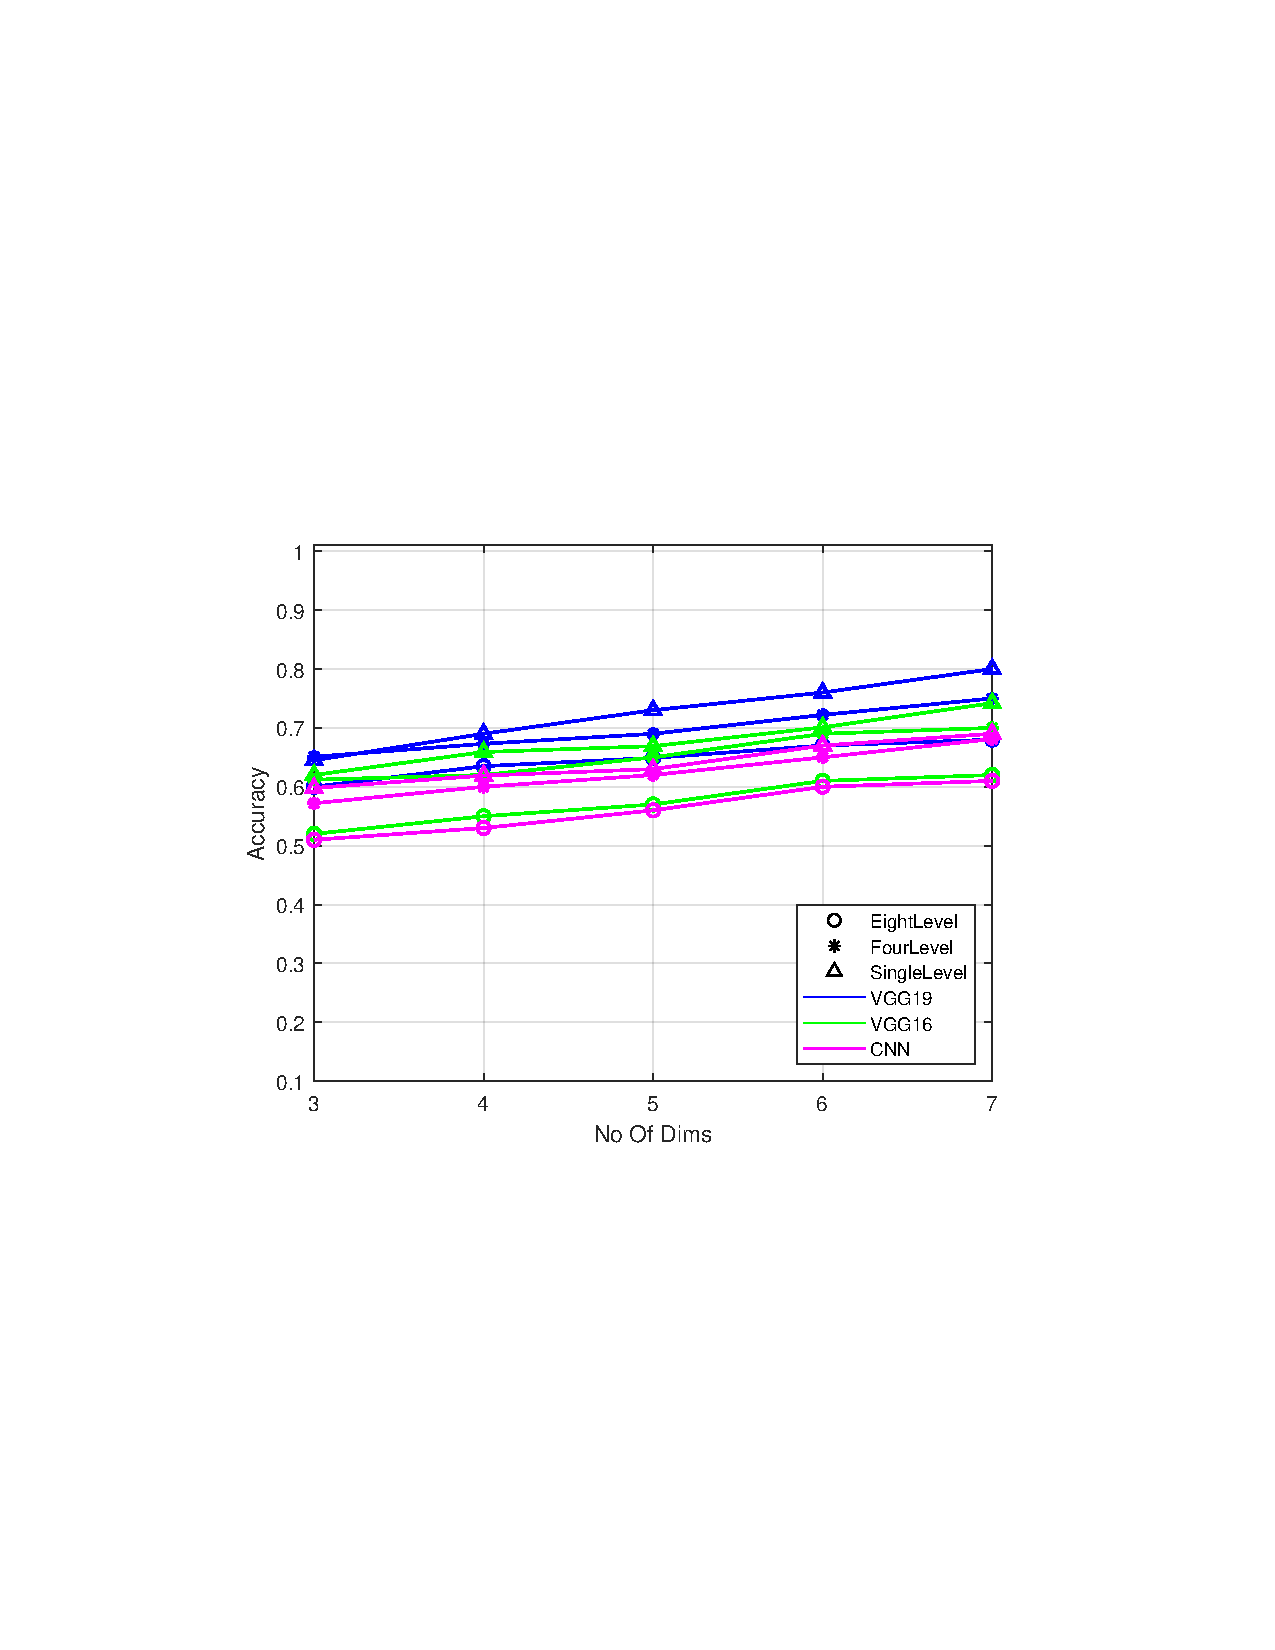
\includegraphics[width=\linewidth, trim=3.8cm 8cm 4cm 8cm, clip=true]{figures/celeba_acc}
		\captionsetup{justification=centering}
		\caption{CelebA}
		\label{fig:celeba_acc}
	\end{subfigure}
	\caption{Accuracy for Different Number of Reduced Dimensions }
	\label{fig:acc}
\end{figure*}

\begin{figure*}[ht!]
	\begin{subfigure}{.33\textwidth}
		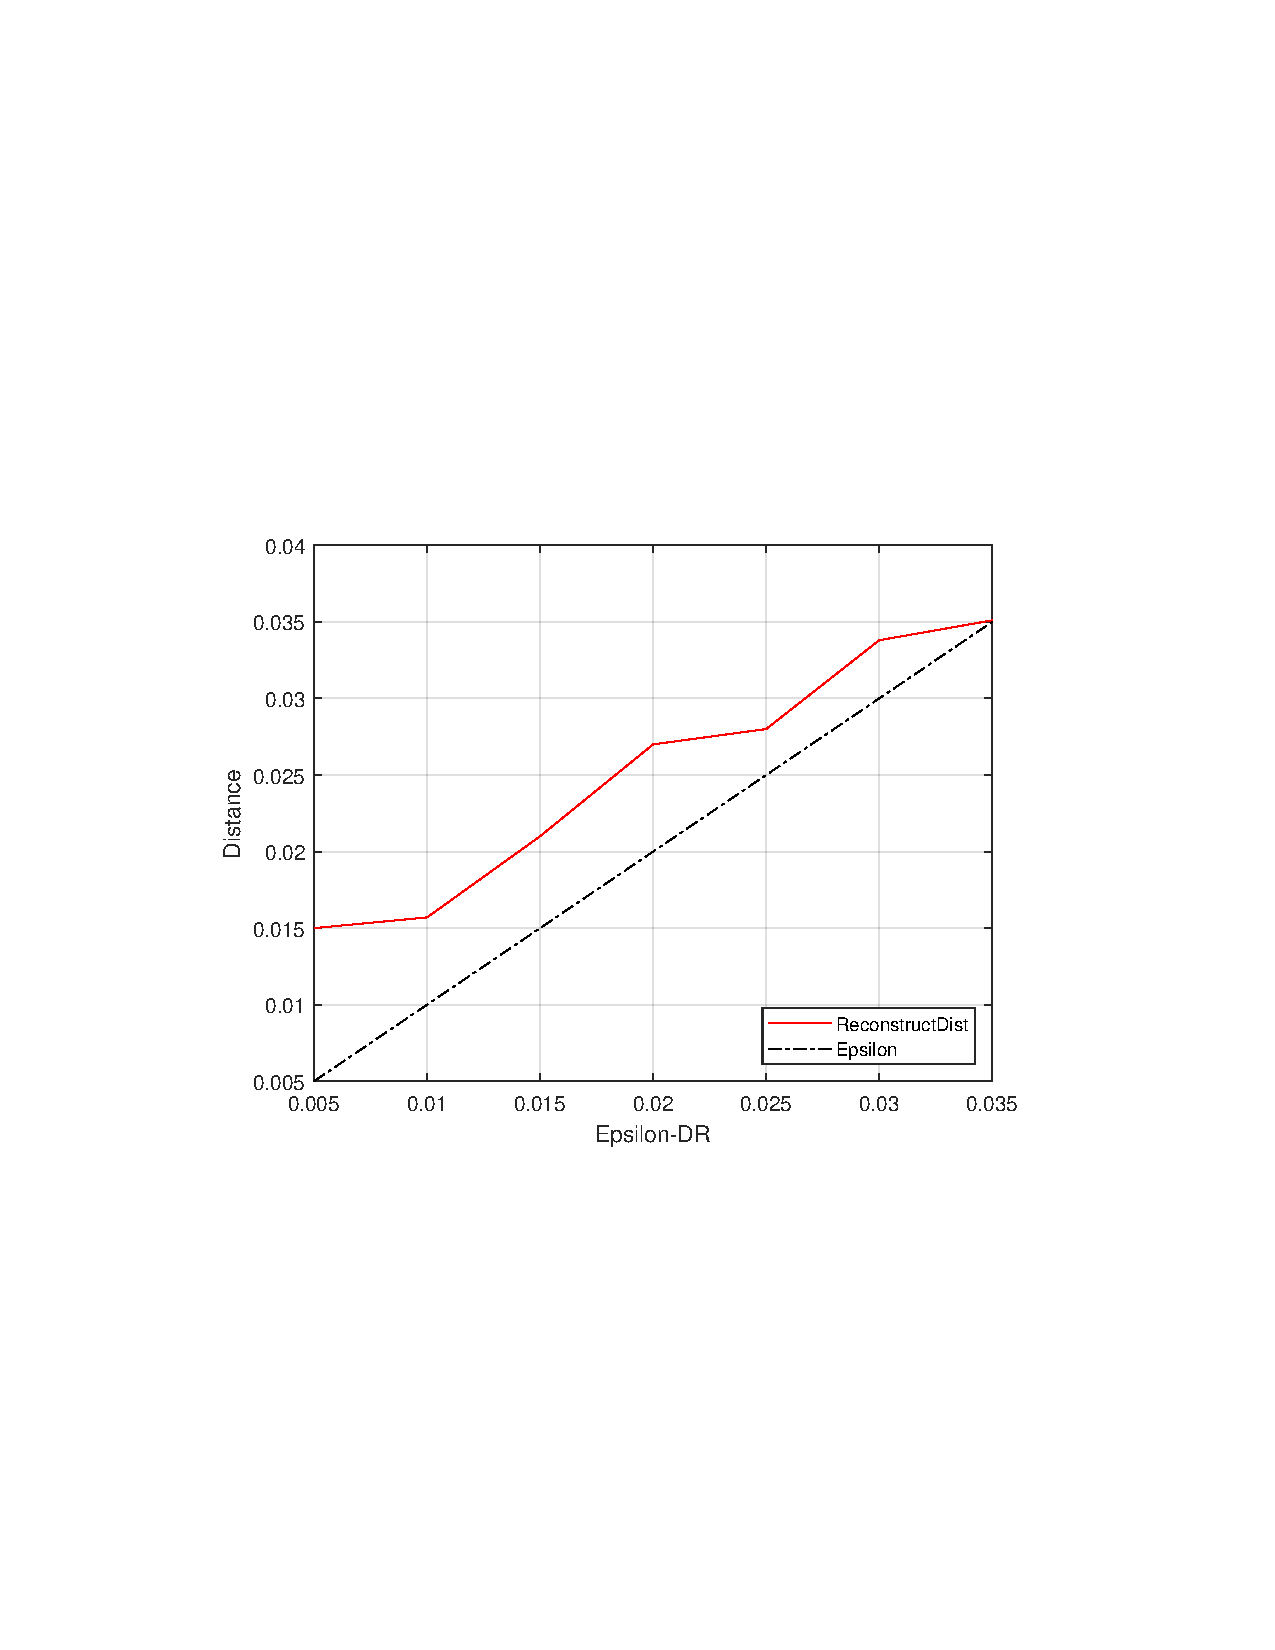
\includegraphics[width=\linewidth, trim=3.8cm 8cm 4cm 8cm, clip=true]{figures/ep_att}
		\captionsetup{justification=centering}
		\caption{ AT\&T}
		\label{fig:att_dist}
	\end{subfigure}
	\begin{subfigure}{.33\textwidth}
		\includegraphics[width=\linewidth, trim=3.8cm 8cm 4cm 8cm, clip=true]{figures/ep_yale}
		\captionsetup{justification=centering}
		\caption{Yale\_B}
		\label{fig:yale_dist}
	\end{subfigure}
	\begin{subfigure}{.33\textwidth}
		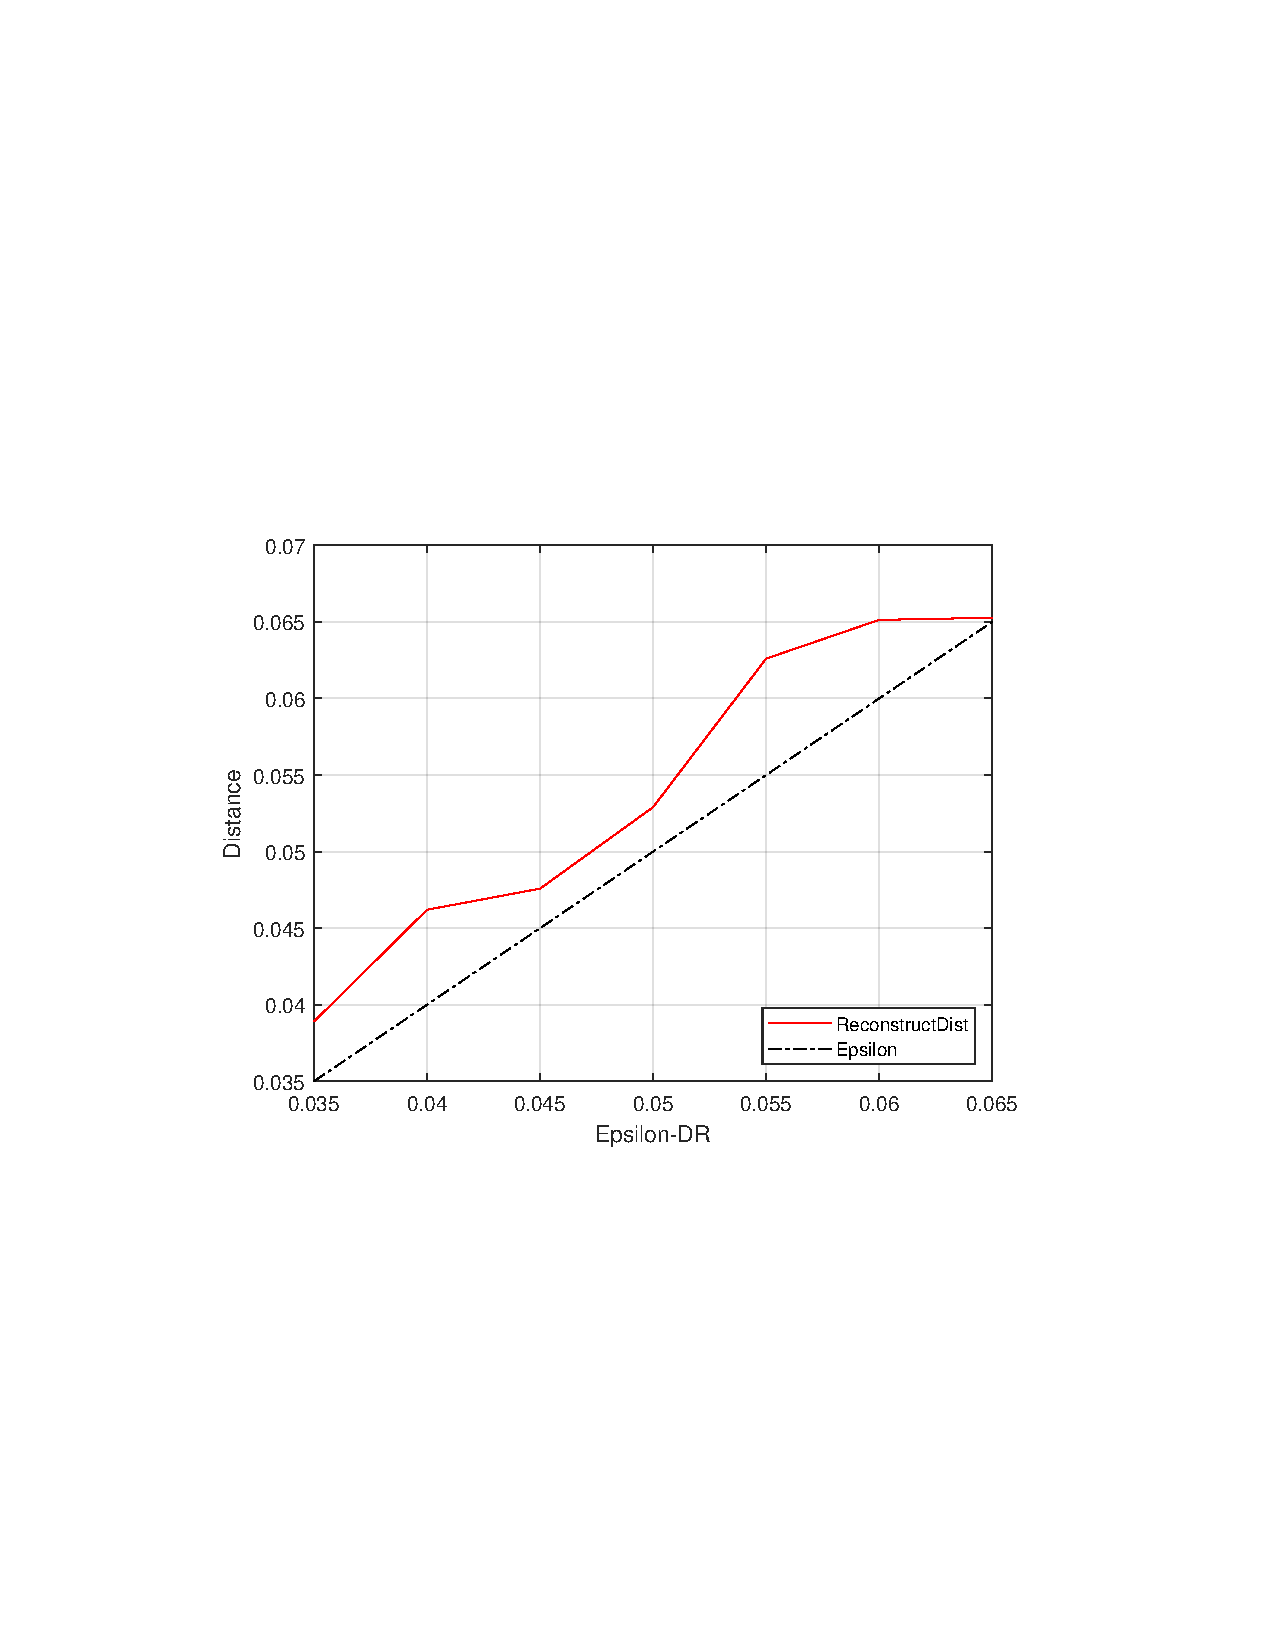
\includegraphics[width=\linewidth, trim=3.8cm 8cm 4cm 8cm, clip=true]{figures/ep_celeba}
		\captionsetup{justification=centering}
		\caption{CelebA}
		\label{fig:celeba_dist}
	\end{subfigure}
	\caption{Average Distance Measurement Result \{ 7 dimensions, Single-Level\}}
	\label{fig:distresult}
\end{figure*}
"


\setcounter{section}{5} "
\section{Visual Comparison to Privacy Preserving Techniques }
\label{AutoGAN_DP_PCA}

In this section, we compare AutoGAN-DRP with other privacy preserving methods in terms of ability to visually identify client's identities. We choose the widely used tool for privacy preserving Differential Privacy (DP) [27] and another privacy preservation method utilizing dimensionality reduction technique (i.e., Principle Component Analysis [34] ).

In these experiments, we implement AutoGAN-DRP following VGG19 structure for the Generator and Re-constructor, and other setting parameters (e.g., number of hidden layers, learning rate, optimization) are shown in Table \ref{table:implementation}. The images are reduced to seven dimensions for different values of $\epsilon$-DR to achieve different distances and accuracies. The datasets are grouped into two groups corresponding to a binary classifier. 

For implementing DP, we first generate a classifier on the authentication server by training the datasets with a VGG19 binary classifier (the structure of hidden layers is similar to our Generator in Table \ref{table:implementation}). The testing images are then perturbed using differential privacy method. Specifically, Laplace noise is added to the images with the sensitivity coefficient of 1 (it is computed by the maximum range value of each pixel [0,1]) and different DP epsilon parameters (this DP epsilon is different from our $\epsilon$-DR). The perturbed images are then sent to the authentication server and fed to the classifier. We visually compare the perturbed images of this method with AutoGAN. 

In addition, we follow instruction in FRiPAL [11] in which the clients reduce image dimension using Principle Component Analysis (PCA) and send reduced features to the server. FRiPAL claims that by reducing image dimension, their method can be more resilient to reconstruction attacks. The experiments are conducted with different number of reduced dimension. The images are reconstructed using \textit{Moore–Penrose inverse} method with assumption that an adversary has assess to the model. The classification accuracy is evaluated using a classifier which has similar structure to AutoGAN's classifier. 

Table \ref{table:visualization} shows image samples and results over the three datasets. Overall, AutoGAN-DRP is more resilient to reconstruction attacks compared to the other two techniques. For instance, at the accuracy of 79\% on AT\&T dataset, 80\% on YaleB, and 73\% on CelebA, we cannot distinguish entities from the others. For DP method, the accuracy decreases when the DP epsilon decreases (adding more noise), and the perturbed images become harder to recognize. However, at a low accuracy 57\%, we are still able to distinguish identities by human eyes. The reason is that DP noise does not focus on the important visual pixels. For PCA, the accuracy also goes down when the number of dimensions decreases and the distances increase. Since PCA transformation is linear and deterministic, the original information can be significantly reconstructed using the inverse transformation deriving from the model or training data. Thus, at the accuracy of 75\% on AT\&T, 71\% on YaleB, and 68\% on CelebA, we still can differentiate individuals. Overall, our proposed method shows the advantage in securing the data while retaining high data utility.       
\\ 
\setcounter{table}{1}

\begin{table}[H]
	\centering
	%trim  left, bottom, right and top 
	\includegraphics[width=0.8\linewidth, trim=1cm 3cm 1cm 3cm, clip=true]{tables/img_table}
	\caption{Sample visualization of AutoGAN, DP, PCA over three datasets}
	\label{table:visualization}
\end{table}

"

\color{blue}
\underline{Comment 3.3} 
Overall, the paper is not well written, please propose a comprehensive revision

\color{black}
\underline{Response:}

Thank you for the suggestion. In this revision, we thoroughly revised the manuscript and made several changes to improve the quality of the manuscript. The main changes can be summarized as follows. 

\begin{enumerate}
	\item The language in a number of sections including Abstract, Introduction, Related work, and Methodology have been revised to improve reading comprehension. 
	
	\item Preliminaries section was merged to Related Work. Problem section and $\epsilon$-Dimension Reduction Privacy section were merged to Methodology. 
	
	\item Section 2 (Related Work) was thoroughly revised to update our references with more latest work (around 10 most recent works were added).
	
	\item Section 3.1.1 (Problem Statement) was revised to give more information about the problem and the sample scenario. 
	
	\item  Figures and tables are rearranged to improve the readability.
	
	\item Conducting more experiments with different structure of AutoGAN-DRP (i.e., VGG19, VGG16, basic CNN were applied to Generator and Re-constructor). Results were updated in Section 4.  
	
	\item Implementing AutoGAN-DRP on one more color dataset (CelebA). Experiment results and discussion in Section 4 were updated correspondingly. 
	
	\item Table 1 (Implementation information) in Section 4 was added to provide precise implementation information of components' structure in Section 4 (Experiment and Discussion)  
	
	\item Section 6 was added, and new experiments were conducted to compare AutoGAN-DRP to other privacy preservation techniques using Differential Privacy (DP) and Principle Component Analysis (PCA). 
	
	\item Table 2 (Sample visualization of AutoGAN, DP, PCA over three datasets) in Section 6 was added to show more intuitive results of AutoGAN, DP, PCA based techniques.   
\end{enumerate}


\end{document}